\documentclass[11pt,reqno]{amsart}
\usepackage[T1]{fontenc}
\usepackage{lmodern}
\usepackage{amsmath,amssymb,amsthm,mathtools}
\usepackage[kerning=true]{microtype}
\usepackage{enumitem,booktabs,graphicx,xcolor}
\usepackage[a4paper,margin=1.12in]{geometry}
\usepackage{placeins}
\graphicspath{{./}{figures/}}
\usepackage{xurl}
\usepackage[colorlinks=true,linkcolor=blue!55!black,citecolor=blue!55!black,
urlcolor=blue!55!black]{hyperref}
\hypersetup{pdftitle={Superlinear Wire Lower Bounds toward P versus NP},pdfauthor={Deep Bhattacharjee}}
\emergencystretch=2em
\numberwithin{equation}{section}
\raggedbottom
\theoremstyle{plain}
\newtheorem{theorem}{Theorem}[section]
\newtheorem{lemma}[theorem]{Lemma}
\newtheorem{proposition}[theorem]{Proposition}
\newtheorem{corollary}[theorem]{Corollary}
\newtheorem*{theoremA}{Theorem A}
\newtheorem*{theoremB}{Theorem B}
\newtheorem*{theoremC}{Theorem C}
\newtheorem*{theoremD}{Theorem D}
\theoremstyle{definition}
\newtheorem{definition}[theorem]{Definition}
\theoremstyle{remark}
\newtheorem{remark}[theorem]{Remark}
\newtheorem{example}[theorem]{Example}
\DeclareMathOperator{\poly}{poly}
\DeclareMathOperator{\SIZE}{SIZE}
\DeclareMathOperator{\NTIME}{NTIME}
\DeclareMathOperator{\DTIME}{DTIME}
\DeclareMathOperator{\thr}{thr}
\DeclareMathOperator{\ex}{ex}
\DeclareMathOperator{\md}{mod}
\DeclareMathOperator{\wires}{w}
\newcommand{\Z}{\mathbb{Z}}
\newcommand{\Q}{\mathbb{Q}}
\newcommand{\N}{\mathbb{N}}
\newcommand{\F}{\mathbb{F}}
\newcommand{\cO}{\mathcal{O}}
\newcommand{\cK}{\mathcal{K}}
\newcommand{\cA}{\mathcal{A}}
\newcommand{\cN}{\mathcal{N}}
\newcommand{\Pc}{\mathsf{P}}
\newcommand{\NP}{\mathsf{NP}}
\newcommand{\coNP}{\mathsf{coNP}}
\newcommand{\ENP}{\mathsf{E}^{\mathsf{NP}}}
\newcommand{\Ec}{\mathsf{E}}
\newcommand{\NEXP}{\mathsf{NEXP}}
\newcommand{\ACC}{\mathsf{ACC}^0}
\newcommand{\AC}{\mathsf{AC}^0}
\newcommand{\TC}{\mathsf{TC}^0}
\newcommand{\Ppoly}{\mathsf{P}/\mathsf{poly}}
\newcommand{\Wl}{\mathsf{W}}
\newcommand{\oai}{OpenAI}
\newcommand{\vtwo}{v_2}
\newcommand{\Darr}{D_{\mathrm{arr}}}
\newcommand{\zenodoDOI}{10.5281/zenodo.0000000}

\title[Superlinear wire lower bounds]{Superlinear Wire Lower Bounds toward P versus NP}
\author{Deep Bhattacharjee}
\address{Electro-Gravitational Space Propulsion Laboratory (EGSPL), Bhubaneswar, Odisha 751030, India}
\address{Formerly, University of Calcutta (Heramba Chandra College), 23/49 Gariahat Road, Golpark, Kolkata 700029, West Bengal, India}
\email{d.bhattacharjee@erl-forschung.de}
\email{itsdeep@live.com}
\email{egspl@proton.me \textup{(GitHub-related contact, \url{https://github.com/creelie})}}
\urladdr{https://orcid.org/0000-0003-0466-750X}
\thanks{Corresponding author: Deep Bhattacharjee, d.bhattacharjee@erl-forschung.de.}
\date{4 November 2026}

\begin{document}

\begin{abstract}
The satisfying inputs of a Boolean circuit with $s$ inputs and wires in all
can be counted in time $2^{O(s/\sqrt{\log s})}$ when every gate is either an
arbitrary function of at most $s^{4/5}$ inputs or a threshold, exact, modular or
symmetric gate of any fan-in with weights of at most $s^{2/3}$ bits.
Consequently a language in $\ENP$ needs more than $cN\sqrt{\log N}$ wires in
circuits on $N$ inputs built from such gates, with arbitrary gates of at most
$N^{3/4}$ inputs and weights of at most $N^{1/2}$ bits. The
$\Pc$ versus $\NP$ problem remains open; we survey where these bounds stand
within it.

\medskip
\noindent\textbf{Keywords:} P versus NP; circuit lower bounds; tensor networks.

\noindent\textbf{MSC 2020:} 68Q17; 68Q15, 68Q25, 68W40, 03D15.
\end{abstract}

\maketitle
\setcounter{tocdepth}{1}
\tableofcontents

%%==================================================================
\section{Introduction}\label{sec:intro}
%%==================================================================

\subsection{The problem}
The class $\Pc$ consists of the languages decided by a deterministic Turing
machine in time polynomial in the input length, and $\NP$ of those decided by a
nondeterministic one in polynomial time, equivalently those whose members have
certificates of polynomial length that can be checked in polynomial time. The
question whether $\Pc=\NP$ was isolated by Cook \cite{Coo71} and Levin
\cite{Lev73}, who showed that satisfiability of propositional formulas is
$\NP$-complete; Karp \cite{Kar72} then showed that twenty-one combinatorial
problems share this property. The question had been anticipated by Edmonds
\cite{Edm65}, who proposed polynomial running time as the mark of an efficient
algorithm, and by G\"odel in a letter of 1956 to von Neumann, discussed by Sipser
\cite{Sip92}. It is one of the seven Millennium Prize Problems of the Clay
Mathematics Institute \cite{Clay}, and the surveys of Sipser \cite{Sip92},
Fortnow \cite{For09}, Aaronson \cite{Aar16} and Wigderson \cite{Wig19} describe
its place in mathematics.\footnote{Gasarch's third poll of researchers
\cite{Gas19}, taken in 2019, found that 88\% of those who answered expected
$\Pc\ne\NP$, against 83\% in 2012 and 61\% in 2002.}

No proof that $\Pc\ne\NP$, or that $\Pc=\NP$, is known, and this paper does not
give one. Its subject is the strongest kind of statement that is currently
within reach: lower bounds for explicit languages against restricted models of
computation. The most direct route to $\Pc\ne\NP$ is to show that some language
in $\NP$ has no Boolean circuits of polynomial size. Shannon \cite{Sha49}
showed that almost every Boolean function of $n$ inputs needs at least
$2^n/(2n)$ gates of fan-in two, yet for languages in $\Pc$, and even in $\NP$,
the best lower bound known is $3.1n-o(n)$ \cite{LY22}, linear in the input
length $n$.\footnote{Throughout, an \emph{explicit} function is one computed
in polynomial time, or at least in exponential time with an $\NP$ oracle; a
lower bound for a function defined by counting, as in Shannon's argument, does
not name the function.} Climbing to $\ENP$, the class of languages decided in
time $2^{O(n)}$ with an oracle for $\NP$, does not help by itself: before the
preprint \cite{OAI26} discussed below, no superlinear lower bound was known for
$\ENP$ even for circuits of fan-in-two gates, and against circuits of larger
gates and unbounded depth nothing superlinear in the number of wires was known
for any language in $\ENP$.

\subsection{What is proved}
In October 2026 \oai{} released a preprint \cite{OAI26} with a deterministic
algorithm that counts the satisfying assignments of a $k$-CNF with $n$ variables
in time $2^{O(n\log\log n/\sqrt{\log n})}$, refuting the exponential time
hypothesis of Impagliazzo and Paturi \cite{IP01}. The algorithm rests on a
contraction theorem for Boolean tensor networks \cite[Theorem D.1]{OAI26},
stated here as Theorem~\ref{thm:contraction}, and \cite[Corollary 1.4]{OAI26}
combines it with Williams' argument \cite{Wil13} to show that a language in
$\ENP$ has no circuits of $c\,n\sqrt{\log n}$ fan-in-two gates. The results
below extend both from fan-in two to gates of large fan-in. Write $\wires(C)$
for the number of wires of a circuit $C$, the sum of the fan-ins of its gates,
and $s(C)=m+\wires(C)$ when $C$ has $m$ inputs.

For integers $F,\beta\ge 1$ let $\cK(F,\beta)$ be the circuits whose gates are of
two kinds (Definition~\ref{def:gates}):
\begin{itemize}[leftmargin=2em]
\item \emph{table gates} computing an arbitrary Boolean function of at most $F$
inputs, given by its truth table;
\item \emph{weighted gates} of any fan-in $f$, computing $\varphi(\sum_i
w_iy_i)$ for integer weights $|w_i|\le 2^{\beta}$, where $\varphi$ is a
threshold $[v\ge\theta]$, an exact test $[v=\theta]$, a congruence
$[v\equiv\theta\bmod\mu]$ with $1\le\mu\le2^\beta$, or, when every weight is
one, an arbitrary function of $v\in\{0,\dots,f\}$ given by its table.
\end{itemize}
Gates of fan-in two, unbounded fan-in AND, OR and parity gates, majority and
threshold gates with weights below $2^\beta$, and $\mathrm{MOD}_\mu$ gates are
all of these kinds, in any combination and at any depth.

\begin{theoremA}[Counting, Theorem~\ref{thm:counting}]
There is a deterministic algorithm that, given a circuit $C\in\cK(s^{4/5},s^{2/3})$
with $s=s(C)\ge 2$, described by $L$ bits, computes the number of inputs on which
$C$ outputs one in time $(s+L)^{O(1)}2^{O(s/\sqrt{\log s})}$ and space
$(s+L)^{O(1)}$. Since $L\le s^{O(1)}2^{s^{4/5}}$, the time is
$2^{O(s/\sqrt{\log s})}$.
\end{theoremA}

\begin{theoremB}[Lower bound, Theorem~\ref{thm:lower}]
There are a language $\Wl\in\ENP$ and a constant $c>0$ such that, for
infinitely many $N$, every circuit in $\cK(N^{3/4},N^{1/2})$ with $N$ inputs
that decides $\Wl$ on inputs of length $N$ has more than $cN\sqrt{\log N}$ wires.
\end{theoremB}

A fan-in-two circuit with $g$ gates has at most $2g$ wires, so Theorem~B
contains \cite[Corollary 1.4]{OAI26}. Table gates of fan-in $N^{3/4}$ cannot be
replaced by fan-in-two gates at linear cost: most functions of $k=N^{3/4}$
inputs need at least $2^k/(2k)$ such gates \cite{Sha49}. A threshold gate of
fan-in $f$ with weights of $\beta$ bits is computed by the usual adder circuits
with $O(f\beta)$ fan-in-two gates, which for $\beta=N^{1/2}$ is far from linear
in its $f$ wires. Theorem~A therefore works with the gates themselves rather
than through a simulation.

The counting theorem also applies to integer programs. For a matrix $A$ write
$\nu(A)$ for its number of nonzero entries.

\begin{theoremC}[Zero-one programs, Corollary~\ref{cor:ilp}]
Let $A\in\Z^{r\times n}$ and $b\in\Z^r$, and put $\sigma=n+\nu(A)$. If every
entry of $A$ has absolute value at most $2^{\sigma^{2/3}}$, the number of
$x\in\{0,1\}^n$ with $Ax\le b$ can be computed in time
$L^{O(1)}2^{O(\sigma/\sqrt{\log\sigma})}$, and a linear objective with
coefficients of the same size can be maximised over these points within the
same bound.
\end{theoremC}

For sparse programs, with $\nu(A)=O(n)$, this is $2^{O(n/\sqrt{\log n})}$.
Before \cite{OAI26}, the best algorithm for zero-one programs with $O(n)$
constraints ran in time $2^{(1-\epsilon)n}$ for a constant $\epsilon>0$
depending on the ratio of constraints to variables \cite{ILPS14}; a
subexponential algorithm for sparse zero-one programs would already have refuted
the exponential time hypothesis, since $3$-SAT with $O(n)$ clauses is such a
program.

The argument that turns Theorem~A into Theorem~B works for any exponent. Its
general form is Theorem~\ref{thm:transfer}:

\begin{theoremD}[Transfer]
Let $\gamma>0$ be rational. If satisfiability of circuits in $\cK(s^{4/5},s^{2/3})$ with
$s$ wires and inputs can be decided in time $L^{O(1)}2^{O(s/(\log s)^\gamma)}$,
then some language in $\ENP$ needs more than $cN(\log N)^\gamma$ wires in
$\cK(N^{3/4},N^{1/2})$ for infinitely many $N$.
\end{theoremD}

Theorem~A supplies $\gamma=\tfrac12$, and a $2^{O(s/\log s)}$ algorithm would
give $cN\log N$. Superpolynomial lower bounds are a different matter. In
Williams' theorem \cite{Wil13} what has to be beaten is exhaustive search over
the $n$ inputs: deciding satisfiability of circuits of polynomial size with $n$
inputs in time $2^n/n^{\omega(1)}$ would show $\NEXP\not\subseteq\Ppoly$. The
bound of Theorem~A is measured in the size $s$, and it is below $2^n$ only while
$s=O(n\sqrt{\log n})$. Section~\ref{sec:limits} explains why the method stops
at $\sqrt{\log N}$ and what each further step would require; none of these
steps would separate $\Pc$ from $\NP$.

\subsection{Plan}
Part~I surveys the problem. Section~\ref{sec:history} gives definitions, history
and equivalent forms; Section~\ref{sec:barriers} the three barriers that every
proof must pass; Section~\ref{sec:circuits} the circuit lower bounds known
today; Section~\ref{sec:algorithms} the algorithmic method, the exponential time
hypothesis and its refutation; Section~\ref{sec:otherroutes} the other
programmes; and Section~\ref{sec:repositories} the repositories and the
catalogue of 6,480 arXiv papers assembled for this survey. Part~II contains the
new results: circuits and tensor networks in Section~\ref{sec:networks},
Theorem~A in Section~\ref{sec:counting}, zero-one programs in
Section~\ref{sec:ilp}, Theorems~B and~D in Section~\ref{sec:lower}, and the
limits of the method in Section~\ref{sec:limits}.
Appendix~\ref{app:contraction} reproduces the proof of the contraction theorem
of \oai{} \cite[Appendix D.4]{OAI26} on which Theorem~A rests, so that the paper
is complete, and Appendix~\ref{app:checks} describes the programs that check its
finite identities.

\subsection*{Conventions}
Logarithms are to base two unless written $\ln$. $[n]=\{1,\dots,n\}$. For a
proposition $P$, $[P]$ is $1$ if $P$ holds and $0$ otherwise. For an integer or
rational number $x\ne0$, $\vtwo(x)$ is its two-adic valuation. Running times
count bit operations on a random-access machine unless a Turing machine is named.

\part{The problem and the state of knowledge}

%%==================================================================
\section{Definitions, history and equivalent forms}\label{sec:history}
%%==================================================================

\subsection{Time, nondeterminism and reductions}
Hartmanis and Stearns \cite{HS65} measured the difficulty of a problem by the
running time of the best Turing machine that decides it and proved the first
hierarchy theorem: for time-constructible $t$, more time decides more
languages. A nondeterministic machine may branch at each step and accepts when
some branch accepts. The class $\NP=\bigcup_k\NTIME(n^k)$ is the set of
languages $\mathcal L$ for which there are a polynomial $p$ and a polynomial-time
relation $R$ with
\[
x\in\mathcal L\iff \exists y\in\{0,1\}^{p(|x|)}\ R(x,y).
\]
The string $y$ is a \emph{certificate}. A polynomial-time \emph{reduction} from
$\mathcal L$ to $\mathcal L'$ is a polynomial-time map $g$ with $x\in\mathcal
L\iff g(x)\in\mathcal L'$, and $\mathcal L'$ is $\NP$-complete if it lies in
$\NP$ and every language in $\NP$ reduces to it.

Cook \cite{Coo71} and, independently, Levin \cite{Lev73} proved that the
satisfiability of propositional formulas is $\NP$-complete.\footnote{Levin's
note treats search problems (``universal sequential search problems'') and
gives six complete ones, among them tiling and set cover; Cook works with
decision problems and Turing reductions. Karp's reductions are the many-one
reductions used today.} The proof writes the computation of a nondeterministic
machine on $x$ as a table of $p(|x|)^2$ cells and expresses its correctness by
clauses that each read a bounded window of the table. Karp \cite{Kar72} reduced
satisfiability to twenty-one problems of combinatorics and optimisation,
including clique, vertex cover, Hamiltonian cycle, three-dimensional matching,
knapsack and zero-one integer programming, and Garey and Johnson \cite{GJ79}
catalogued several hundred more. Consequently $\Pc=\NP$ if and only if any one
of these problems has a polynomial-time algorithm.

Edmonds \cite{Edm65} had argued, in his paper on matchings, that polynomial time
is the right notion of a ``good'' algorithm. G\"odel asked von Neumann in 1956 whether
the existence of proofs of length $n$ for a given formula can be decided in time
linear or quadratic in $n$, which is the bounded form of the same question; the
letter is translated and discussed by Sipser \cite{Sip92}.

\subsection{What is known to separate}
Diagonalisation separates classes defined by the same resource at different
amounts. The deterministic hierarchy of Hartmanis and Stearns, and the
nondeterministic hierarchies of Cook \cite{Coo73}, Seiferas, Fischer and Meyer
\cite{SFM78} and \v{Z}\'ak \cite{Zak83}, show for instance
$\NTIME(2^n)\ne\NTIME(2^{n/2})$; \v{Z}\'ak's form, which separates unary
languages, is the one used in Section~\ref{sec:lower}. Between different
resources very little is separated. Paul, Pippenger, Szemer\'edi and Trotter
\cite{PPST83} proved $\DTIME(n)\ne\NTIME(n)$ for multitape machines, a statement
that does not extend to $n^k$. Hopcroft, Paul and Valiant \cite{HPV77} showed
that time $t$ can be simulated in space $t/\log t$, and Williams \cite{Wil25}
improved this to space $\sqrt{t\log t}$. Fortnow, Lipton, van Melkebeek and
Viglas \cite{FLMV05} proved that satisfiability cannot be decided
simultaneously in time $n^c$ and space $n^{o(1)}$ for any $c$ below the golden
ratio.

For space, nondeterminism costs at most a square: Savitch \cite{Sav70} proved
that nondeterministic space $s$ is contained in deterministic space $s^2$, so
$\mathsf{PSPACE}=\mathsf{NPSPACE}$. No analogue is known for time; the best
deterministic simulation of $\NTIME(t)$ takes time $2^{O(t)}$.

\subsection{Structure inside $\NP$}
If $\Pc\ne\NP$, Ladner \cite{Lad75} showed that $\NP$ contains problems that are
neither in $\Pc$ nor $\NP$-complete. Some natural problems were long thought to
be of this kind; primality was placed in $\Pc$ by Agrawal, Kayal and Saxena
\cite{AKS04}. Counting is much stronger than deciding: Valiant \cite{Val79b}
proved the permanent of a zero-one matrix $\#\Pc$-complete although the
corresponding decision problem, existence of a perfect matching, is in $\Pc$,
and Toda \cite{Tod91} showed that the whole polynomial hierarchy reduces to
$\#\Pc$. The PCP theorem of Arora and Safra \cite{AS98} and of Arora, Lund,
Motwani, Sudan and Szegedy \cite{ALMSS98}, with Dinur's combinatorial proof
\cite{Din07}, shows that every language in $\NP$ has certificates that a
randomised verifier checks by reading a constant number of bits; equivalently,
approximating the maximum fraction of satisfiable clauses of a $3$-CNF within
some constant factor is already $\NP$-hard. Impagliazzo \cite{Imp95} described
five possible worlds, from $\Pc=\NP$ to the existence of public-key
cryptography, that are consistent with present knowledge.

\subsection{Circuits}
A Boolean circuit with $n$ inputs is a directed acyclic graph whose sources are
the inputs and whose other vertices, the gates, compute Boolean functions of
their predecessors. The \emph{size} of a circuit over the binary basis is its
number of gates; for gates of larger fan-in the right measure is the number of
\emph{wires}, the sum of the fan-ins. A language $\mathcal L$ has circuits of
size $s(n)$ if for each $n$ some circuit of that size decides $\mathcal L$ on
inputs of length $n$; the class $\Ppoly$ consists of the languages with
circuits of polynomial size. Since $\Pc\subseteq\Ppoly$, a proof that some
language in $\NP$ lies outside $\Ppoly$ would prove $\Pc\ne\NP$. The circuit
form is attractive because it removes uniformity, so that only combinatorics
remains, and because $\NP\not\subseteq\Ppoly$ is believed to be true for
satisfiability itself. Kannan \cite{Kan82} proved that $\Sigma_2\Pc$ is not
contained in $\SIZE(n^k)$ for any fixed $k$, and Santhanam \cite{San09}
proved the same for Merlin--Arthur languages with one bit of advice.

\subsection{The Millennium Problem}
The Clay Mathematics Institute listed the question among its seven Millennium
Prize Problems in 2000 \cite{Clay}; the official problem description is by
Cook. Fortnow \cite{For09} and Aaronson \cite{Aar16} survey the evidence,
Wigderson \cite{Wig19} places it within mathematics as a whole, and the
textbooks of Arora and Barak \cite{AB09} and of Jukna \cite{Juk12} give the
technical background used below. Gasarch's polls \cite{Gas19} record a
steadily growing majority of researchers who expect $\Pc\ne\NP$.

%%==================================================================
\section{Three barriers}\label{sec:barriers}
%%==================================================================

Three theorems show that the methods that settle other questions cannot settle
this one by themselves. Each barrier is a statement about proofs, and each has
been circumvented in some restricted setting.

\subsection{Relativization}
Baker, Gill and Solovay \cite{BGS75} constructed oracles $A$ and $B$ with
$\Pc^A=\NP^A$ and $\Pc^B\ne\NP^B$. Any argument that treats machines as black
boxes, such as diagonalisation and simulation, gives the same answer relative
to every oracle and therefore cannot decide the question. The hierarchy
theorems relativize; the Cook--Levin theorem, which uses the local structure of
computations, does not relativize in its strong forms, and the arguments of
Section~\ref{sec:algorithms} use it through local reductions.

\subsection{Natural proofs}
Razborov and Rudich \cite{RR97} observed that the known circuit lower bounds
proceed by a property $\Gamma$ of truth tables that is \emph{useful} (no
function with the property has small circuits), \emph{large} (a fraction
$2^{-O(n)}$ of all functions has it) and \emph{constructive} (it can be
decided in time polynomial in $2^n$ from the truth table). They proved that a
natural property useful against $\Ppoly$ would break pseudorandom functions
that are secure against circuits of size $2^{n^\epsilon}$, whose existence
follows from standard cryptographic assumptions. Arguments by diagonalisation
are not natural, since they single out one function; Williams \cite{Wil16}
showed that $\NEXP\not\subseteq\mathcal C$ is in fact equivalent to the
existence of a property useful against $\mathcal C$ that is constructive in a
weak, nondeterministic sense, which locates the barrier exactly.

\subsection{Algebrization}
Aaronson and Wigderson \cite{AW09} extended relativization to algebraic
oracles, which also capture the arithmetisation used in interactive proofs.
They proved that every known non-relativizing technique of that kind
algebrizes, and that resolving $\Pc$ versus $\NP$ needs non-algebrizing
methods.

\subsection{Locality}
A fourth, newer observation concerns hardness magnification. Oliveira and
Santhanam \cite{OS18}, and earlier Allender and Kouck\'y \cite{AK10}, found
problems for which a slightly superlinear lower bound would imply a
superpolynomial one. Chen, Hirahara, Oliveira, Pich, Rajgopal and Santhanam
\cite{CHOPRS22} proved that the known slightly superlinear lower bounds hold
also for circuits with small oracle gates of unbounded function, while the
magnified statements fail for such circuits; so the methods that prove the weak
bounds cannot prove the magnified ones. This is the \emph{locality barrier}.

\begin{remark}\label{rem:barrierhere}
The lower bound of Theorem~B is proved by diagonalisation against a
nondeterministic class combined with a satisfiability algorithm. It names a
single language, so it is not natural, and it uses the local structure of
computations through the reduction of Lemma~\ref{lem:jmv}.
Section~\ref{sec:limits} discusses its relation to the locality barrier.
\end{remark}

%%==================================================================
\section{Circuit lower bounds known today}\label{sec:circuits}
%%==================================================================

Figure~\ref{fig:landscape} arranges the results of this section by model and
strength.

\begin{figure}[t]
\centering
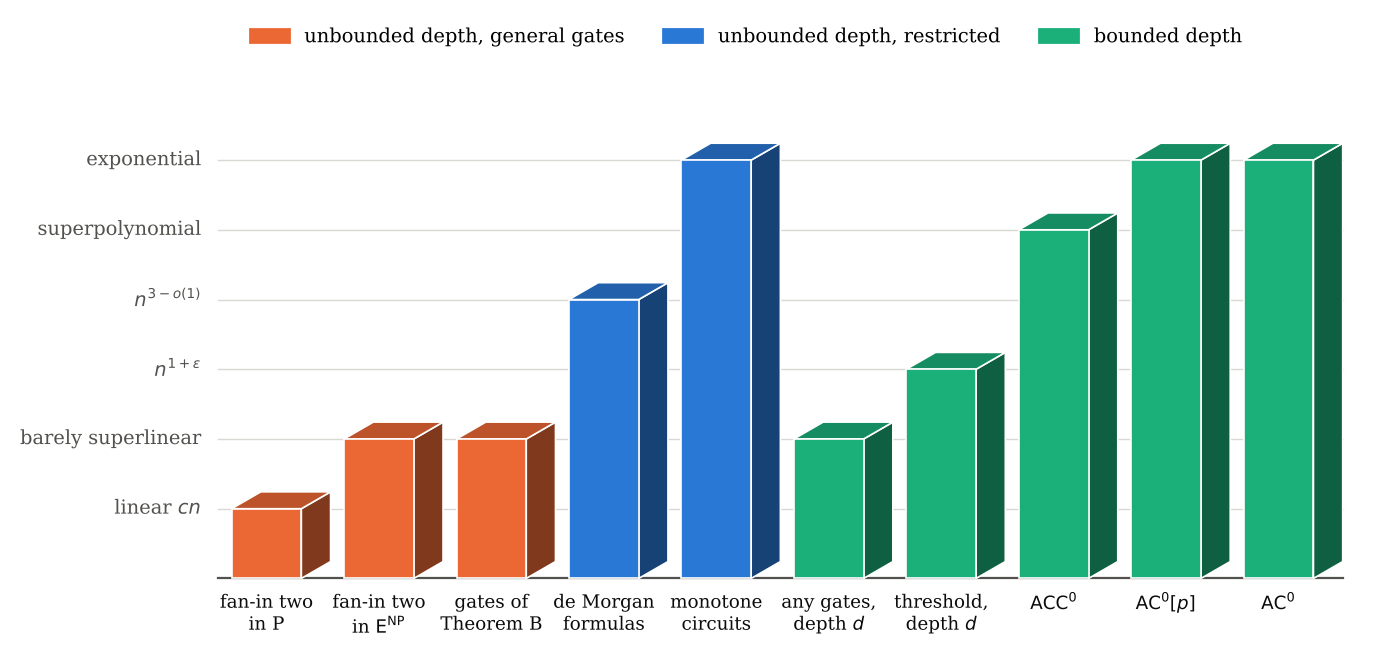
\includegraphics[width=0.92\textwidth]{fig_landscape.png}
\caption{Explicit circuit lower bounds by model. The height of a bar is the
order of growth of the best bound, on a scale from linear ($cn$) to exponential
($2^{n^\epsilon}$); ``barely superlinear'' means $n\cdot\omega(1)$ but
$n^{1+o(1)}$. For circuits of unbounded depth over a complete basis (orange),
only linear bounds were known for explicit languages before \cite{OAI26};
\cite[Corollary 1.4]{OAI26} and Theorem~B give $cn\sqrt{\log n}$. The bounds for
arbitrary gates of bounded depth are for operators with $n$ outputs.}\label{fig:landscape}
\end{figure}

\subsection{General circuits}
Shannon's counting \cite{Sha49} shows that almost every function needs about
$2^n/n$ gates, and Lupanov's construction (see \cite[Chapter 1]{Juk12})
matches this. For explicit functions the only method for unbounded depth has
been gate elimination: fixing an input variable removes a few gates, and
repeating the step $n$ times gives a linear bound. Schnorr \cite{Sch80} and
Blum \cite{Blu84} pushed the constant to three (Schnorr announced $3n$, and
Blum, noting a gap in one lemma, proved $3n-o(n)$ for a modification of Paul's
function), Find, Golovnev, Hirsch and
Kulikov \cite{FGHK16} to $3+\frac1{86}$, and Li and Yang \cite{LY22} to
$3.1n-o(n)$ for a function in $\Pc$.\footnote{Over the de Morgan basis, where
negations are free and the gates are AND and OR, Iwama and Morizumi
\cite{IM02} proved $5n-o(n)$.} Golovnev, Hirsch, Knop and Kulikov
\cite{GHKK18} showed that natural forms of gate elimination cannot prove much
more than linear bounds, and Golovnev, Kulikov, Smal and Tamaki \cite{GKST18}
turned gate elimination into satisfiability algorithms for linear-size
circuits.

\subsection{Formulas}
A formula is a circuit whose gates have fan-out one. Random restrictions
shrink de Morgan formulas: H\aa stad \cite{Has98} proved shrinkage exponent
two, so Andreev's function requires formulas of size $n^{3-o(1)}$, and Tal
\cite{Tal14} sharpened the lower-order terms to a polylogarithmic factor.
Karchmer and Wigderson \cite{KW90} identified formula depth with the
communication complexity of a game; with it they proved that monotone formulas
for connectivity need depth $\Omega(\log^2 n)$, and Raz and McKenzie
\cite{RM99} separated the levels of the monotone $\mathsf{NC}$ hierarchy.

\subsection{Bounded depth}
Ajtai \cite{Ajt83} and Furst, Saxe and Sipser \cite{FSS84} proved that parity is
not in $\AC$, the class of polynomial-size circuits of constant depth with
unbounded fan-in AND and OR gates. Yao \cite{Yao85} and H\aa stad \cite{Has86}
made the bound exponential: depth $d$ requires size $2^{\Omega(n^{1/(d-1)})}$.
Rossman \cite{Ros08} proved that detecting a $k$-clique needs size
$\omega(n^{k/4})$ at every constant depth. With parity gates added, Razborov
\cite{Raz87} and Smolensky \cite{Smo87} proved exponential lower bounds for
majority, and for counting modulo $q$ in circuits with gates modulo a prime
$p\nmid q$.

\subsection{Monotone circuits}
Razborov's method of approximations gave superpolynomial lower bounds for
clique in monotone circuits, made exponential by Alon and Boppana \cite{AB87}
(see \cite[Chapter 9]{Juk12}). Tardos \cite{Tar88} showed that the gap between
monotone and general circuits can be exponential, so monotone bounds do not
transfer.

\subsection{$\ACC$ and the algorithmic method}
For circuits of constant depth with gates counting modulo arbitrary $m$, the
class $\ACC$, no lower bound followed from the methods above. Williams
\cite{Wil14} proved $\NEXP\not\subseteq\ACC$ by a satisfiability algorithm for
$\ACC$ circuits that beats exhaustive search, combined with the argument of
\cite{Wil13} described in Section~\ref{sec:algorithms}. Murray and Williams
\cite{MW20} extended it to nondeterministic quasi-polynomial time, and
Williams \cite{Wil14b} to $\ACC$ circuits with a layer of threshold gates at the
bottom.

\subsection{High classes}
Exponential classes with alternation reach maximum circuit size. Chen,
Hirahara and Ren \cite{CHR24} proved that a language in symmetric exponential
time $\mathsf{S_2E}$ with one bit of advice requires circuits of size about
$2^n/n$, and Li \cite{Li24} removed the advice; this class lies between
$\ENP$ and $\mathsf{ZPE}^{\NP}$ by Cai's theorem \cite{Cai07}. For $\ENP$
itself, whether every language has circuits of linear size was open until
\cite[Corollary C.1]{OAI26}.

\subsection{Threshold circuits}
A threshold gate outputs $[\sum_iw_iy_i\ge\theta]$. Polynomial-size threshold
circuits of constant depth form $\TC$, a class that contains all of the
arithmetic of integers and for which no superpolynomial lower bound is known
even at depth two for functions in $\NEXP$. The known results concern size near
linear. Hajnal, Maass, Pudl\'ak and Szegedy \cite{HMPST93} separated depth two
from depth three for majority circuits. Impagliazzo, Paturi and Saks
\cite{IPS97} proved that parity needs $n^{1+c\theta^{-d}}$ wires in threshold
circuits of depth $d$, for constants $c>0$ and $\theta>1$. Kane and Williams
\cite{KW16} proved superlinear gate and superquadratic wire bounds for depth
two. Chen, Santhanam and Srinivasan \cite{CSS18} proved average-case lower
bounds and satisfiability algorithms for threshold circuits of depth $d$ with
$n^{1+\epsilon_d}$ wires, and Impagliazzo, Paturi and Schneider \cite{IPS13}
gave a satisfiability algorithm for sparse depth-two threshold circuits.
Every one of these bounds degrades with the depth and gives nothing at
unbounded depth.

\subsection{Arbitrary gates}
When gates may compute any function, a single gate of fan-in $n$ computes every
Boolean function, so lower bounds concern either many outputs or bounded fan-in.
For operators with $n$ outputs, Valiant's graph-theoretic method \cite{Val77},
Pudl\'ak's analysis of communication in bounded depth \cite{Pud94}, the bounds
of Radhakrishnan and Ta-Shma for depth-two superconcentrators \cite{RTS00}, and
the explicit operators of Cherukhin \cite{Che11} and Jukna \cite{Juk10} give
superlinear wire bounds that hold only at bounded depth. Theorem~B is a bound of
the second kind: its table gates have fan-in at most $N^{3/4}$ and its depth is
unrestricted.

\subsection{Algebraic circuits}
Valiant \cite{Val79a} introduced the algebraic classes $\mathsf{VP}$ and
$\mathsf{VNP}$ and showed that the permanent is complete for $\mathsf{VNP}$; the
conjecture $\mathsf{VP}\ne\mathsf{VNP}$ is the algebraic analogue of $\Pc\ne\NP$.
Limaye, Srinivasan and Tavenas \cite{LST21} proved the first superpolynomial
lower bounds against algebraic circuits of every constant depth. Kabanets and
Impagliazzo \cite{KI04} showed that derandomising polynomial identity testing
implies lower bounds of this kind, which ties the algebraic question to
pseudorandomness.

\subsection{Range avoidance}
Given a circuit $C:\{0,1\}^n\to\{0,1\}^{n+1}$, find a string outside its range.
Korten \cite{Kor21} showed that this search problem captures explicit
constructions, among them hard truth tables; Ren, Santhanam and Wang
\cite{RSW22} studied its complexity, and Ilango, Li and Williams \cite{ILW23}
connected it to indistinguishability obfuscation. The lower bounds of
\cite{CHR24,Li24} come from an algorithm for range avoidance with an $\NP$
oracle.

%%==================================================================
\section{Algorithms, the exponential time hypothesis and its refutation}\label{sec:algorithms}
%%==================================================================

\subsection{Exponential algorithms for satisfiability}
Exhaustive search decides satisfiability of a formula with $n$ variables in
time $2^n$ times a polynomial. For $k$-CNF formulas much better is known.
Sch\"oning's random walk \cite{Sch99} runs in time $(2-2/k)^n$; the algorithm of
Paturi, Pudl\'ak, Saks and Zane \cite{PPSZ05} improves this, and Hertli
\cite{Her14} proved that its bounds for formulas with a unique solution hold in
general, about $1.308^n$ for $3$-SAT. Williams \cite{Wil05} solved maximum
two-constraint satisfaction in time $2^{\omega n/3}$ by fast matrix
multiplication, where $\omega<2.38$ is the exponent of matrix multiplication.

\subsection{The hypotheses}
Impagliazzo and Paturi \cite{IP01} formulated the \emph{exponential time
hypothesis} (ETH): there is $\delta>0$ such that $3$-SAT cannot be decided in
time $2^{\delta n}$. The \emph{strong} hypothesis (SETH) asserts that for every
$\epsilon>0$ some $k$ makes $k$-SAT require time $2^{(1-\epsilon)n}$.
Impagliazzo, Paturi and Zane \cite{IPZ01} proved the sparsification lemma, by
which ETH is equivalent to the same statement for formulas with $O(n)$
clauses, and Calabro, Impagliazzo and Paturi \cite{CIP06,CIP09} related clause
width to clause density and extended the hypotheses to circuits of small depth.
A large part of fine-grained complexity derives conditional lower bounds from
these hypotheses.

\subsection{Williams' algorithmic method}
Williams \cite{Wil13} proved that a satisfiability algorithm for a circuit
class that is only slightly faster than exhaustive search yields a lower bound
for that class. The argument runs as follows (Figure~\ref{fig:pipeline}).
Suppose that every language in $\NEXP$ has small circuits in the class. By the
easy-witness lemma of Impagliazzo, Kabanets and Wigderson \cite{IKW02}, every
satisfiable instance then has a witness whose bits are computed by a small
circuit. A nondeterministic machine guesses such a circuit, composes it with a
succinct description of the instance, and verifies the witness by running the
fast satisfiability algorithm on the composed circuit. This solves every
language of $\NTIME(2^n)$ in nondeterministic time below $2^n$, contradicting
the nondeterministic hierarchy theorem. The survey \cite{Wil14c} describes the
many variants. The succinct description is a \emph{local reduction}: Jahanjou,
Miles and Viola \cite{JMV15} showed that the clauses of the Cook--Levin formula
for a computation of length $T$ can be indexed by $\log T+O(\log\log T)$ bits
in such a way that each clause is computed from its index by a circuit of
quasi-linear size whose output bits each depend on few index bits.

\begin{figure}[t]
\centering
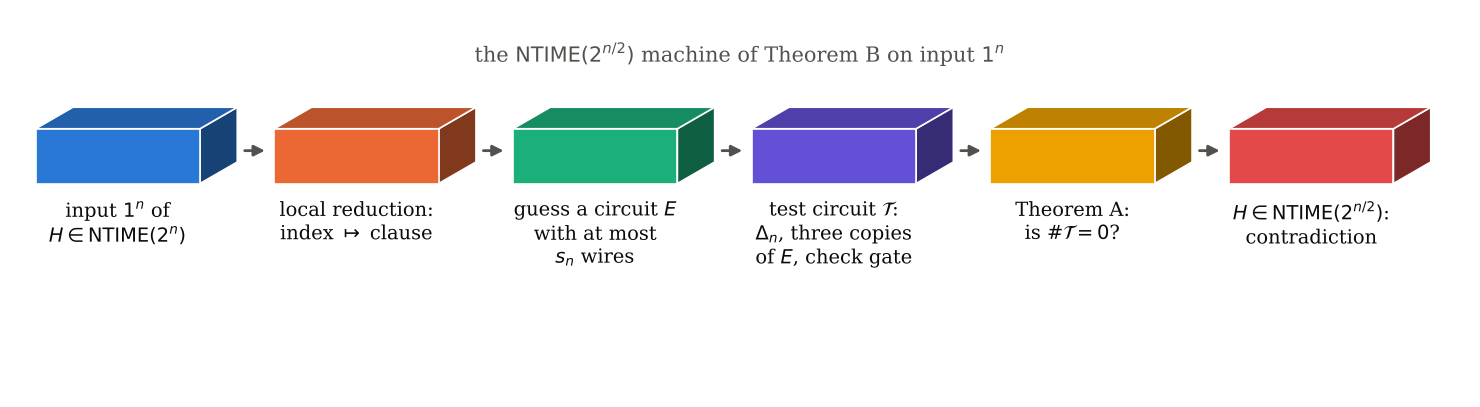
\includegraphics[width=0.92\textwidth]{fig_pipeline.png}
\caption{Williams' argument as used in Section~\ref{sec:lower}. A unary
language that is hard for nondeterministic time $2^{n/2}$ is reduced locally to
a succinct $3$-CNF; a small circuit for the witness language $\Wl$ is guessed,
three copies of it read the variables of an indexed clause, and the test
circuit is checked by the counting algorithm of Theorem~A.}\label{fig:pipeline}
\end{figure}

Santhanam \cite{San10} gave satisfiability algorithms for formulas, Seto and
Tamaki \cite{ST13} for formulas over the full binary basis, and Chen, Kabanets,
Kolokolova, Shaltiel and Zuckerman \cite{CKKSZ15} showed how lower-bound proofs
by restriction yield such algorithms in general.

\subsection{The refutation of ETH}
In October 2026 \oai{} released the preprint \cite{OAI26}, whose main theorem
counts the satisfying assignments of a $k$-CNF with $n$ variables and $m$
clauses in time
\[
(n+m)^{O_k(1)}\,2^{O_k(n\log\log n/\sqrt{\log n})},
\]
and in time $2^{O(n/\sqrt{\log n})}$ when $m=O(n)$. This contradicts ETH, and
with the sparsification lemma it removes the basis of many conditional lower
bounds. The fixed-density bound rests on a theorem about tensor networks,
\cite[Theorem D.1]{OAI26}, restated below as Theorem~\ref{thm:contraction}: a
bipartite Boolean tensor network with $O(s)$ edges and degrees at most
$s^{9/10}$ can be contracted in time $2^{O(s/\sqrt{\log s})}$. Its proof
deforms the identification of the wires by a Cauchy matrix, expands the
interactions between groups of vertices in variables whose two-adic valuations
grow with their weight, and recovers the value at the undeformed point by
Hermite interpolation with tapered multiplicities; Appendix~\ref{app:contraction}
gives the full argument. Contraction of tensor networks had been used for the
simulation of quantum circuits by Markov and Shi \cite{MS08}, with running time
exponential in the treewidth; the theorem of \oai{} needs no bound on the
treewidth.

Combining the fixed-density algorithm with Williams' method, \cite[Corollary
1.4]{OAI26} proves that some language in $\ENP$ needs more than $cn\sqrt{\log
n}$ gates of fan-in two for infinitely many $n$. This was the first superlinear
lower bound of any kind for $\ENP$. Weighted counting, Max-Cut profiles and
exact optimisation follow from the same algorithm \cite{BhaHex26,Bha26eth}.

\subsection{What the refutation does not give}
A subexponential algorithm for $3$-SAT does not place $\NP$ in $\Pc$: the time
$2^{O(n/\sqrt{\log n})}$ is still superpolynomial. Nor does it give a
superpolynomial circuit lower bound, since Williams' method needs an algorithm
whose saving over $2^n$ is measured against the number $n$ of inputs of
circuits of polynomial size, and the algorithms of \cite{OAI26} are fast only
when the circuit has $O(n\sqrt{\log n})$ wires.

%%==================================================================
\section{Other programmes}\label{sec:otherroutes}
%%==================================================================

\subsection{Geometric complexity theory}
Mulmuley and Sohoni \cite{MS01} proposed to separate the permanent from the
determinant, and so $\mathsf{VNP}$ from $\mathsf{VP}$, by representation
theory: the orbit closure of the padded permanent would not be contained in
that of the determinant, and an \emph{obstruction}, an irreducible
representation occurring in the coordinate ring of one closure and not of the
other, would witness this. Mulmuley \cite{Mul12} describes the programme.
B\"urgisser, Ikenmeyer and Panova \cite{BIP19} proved that occurrence
obstructions, those detected by the mere presence of a representation, do not
exist in the required range; obstructions by multiplicities remain possible.

\subsection{Proof complexity}
Cook and Reckhow \cite{CR79} showed that $\NP\ne\coNP$ if and only if no
propositional proof system has polynomial-size proofs of all tautologies; since
$\Pc=\NP$ implies $\NP=\coNP$, superpolynomial lower bounds for every proof
system would separate $\Pc$ from $\NP$. Haken \cite{Hak85} proved that
resolution needs exponential size for the pigeonhole principle, and
Ben-Sasson and Wigderson \cite{BSW01} related resolution size to width.
Kraj\'i\v{c}ek's monograph \cite{Kra19} surveys the field; for Frege systems
no superpolynomial bound is known.

\subsection{Meta-complexity}
The minimum circuit size problem MCSP asks, given a truth table and a number
$s$, whether the function has a circuit of size $s$. Kabanets and Cai
\cite{KC00} began its modern study; it is in $\NP$, and its $\NP$-hardness is open.
Hirahara \cite{Hir18} gave a non-black-box reduction from worst case to average
case for approximating it, and \cite{Hir22} proved $\NP$-hardness of a partial
version. These questions concern the complexity of complexity itself and are
closely tied to natural proofs and to magnification.

\subsection{Hardness versus randomness}
Nisan and Wigderson \cite{NW94} built pseudorandom generators from hard
functions, and Impagliazzo and Wigderson \cite{IW97} proved $\mathsf{P}=
\mathsf{BPP}$ if some language in $\Ec$ requires circuits of size $2^{\Omega(n)}$.
Conversely, derandomization implies lower bounds \cite{KI04,Wil16}. A lower
bound of the strength of Theorem~B is far too weak for derandomization.

\subsection{Magnification}
The results of \cite{AK10,OS18,CHOPRS22} identify problems, many of them
variants of MCSP, for which a lower bound of the form $n^{1+\epsilon}$ in some
model implies a superpolynomial bound in a stronger model. The locality
barrier of Section~\ref{sec:barriers} explains why the known methods have not
reached the magnified thresholds.

%%==================================================================
\section{Repositories and the literature catalogue}\label{sec:repositories}
%%==================================================================

\subsection{Collections of claims}
Woeginger's page \cite{Woe16}, maintained until 2016, lists the announced
solutions that came to his attention, with entries dated from 1986 to 2016.
Parsing the page gives 114 entries with a stated verdict: 62 claim $\Pc=\NP$, 49 claim $\Pc\ne\NP$, two
claim that the question is unprovable and one that it is undecidable
(Figure~\ref{fig:claims}). None has been accepted. The first entry already
illustrates a lesson that became a theorem: polynomial linear programs for the
travelling salesman problem were refuted by Yannakakis \cite{Yan91}, who
proved that every symmetric linear program expressing the problem has
exponential size.

\begin{figure}[t]
\centering
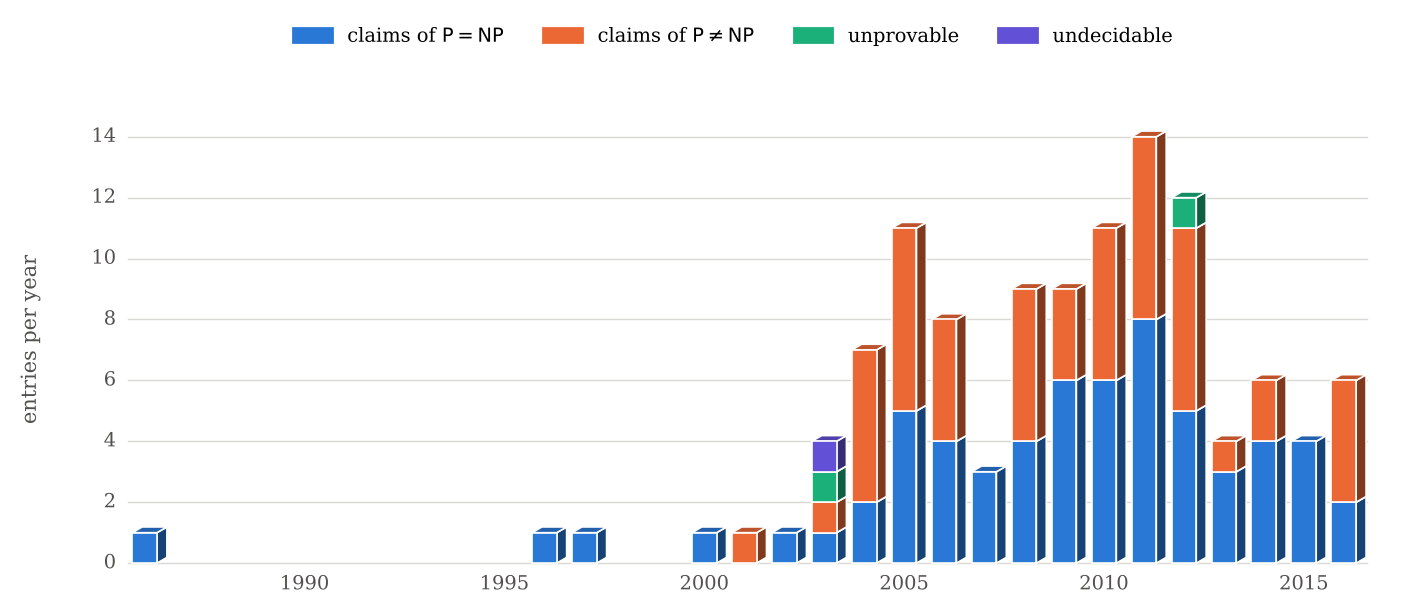
\includegraphics[width=0.9\textwidth]{fig_claims.png}
\caption{Announced solutions of the $\Pc$ versus $\NP$ problem listed by
Woeginger \cite{Woe16}, by year and verdict (114 dated entries). None of them
is accepted.}\label{fig:claims}
\end{figure}

\subsection{Archives}
The Electronic Colloquium on Computational Complexity \cite{ECCC} and the
Complexity Zoo \cite{Zoo}, a catalogue of several hundred complexity
classes and their known inclusions, are the standard reference points. The
preprint \cite{OAI26} and its Lean formalisation are in the public repository
of \oai{}. Archived code accompanies the author's related papers on counting
\cite{Bha26eth}, on Weil classes \cite{Bha26weil} and on Tate--Shafarevich
groups \cite{Bha26bsd}; the programs that check the finite identities of this
paper are archived in the same way (Declarations).

\subsection{A catalogue of arXiv papers}
To measure the field, nineteen keyword queries were run against the arXiv
interface, one for each topic of Sections~\ref{sec:history}
to~\ref{sec:otherroutes}: $\Pc$ versus $\NP$, circuit lower bounds, natural
proofs, relativization, algebrization, geometric complexity theory, hardness
magnification, MCSP, meta-complexity, proof complexity, the exponential time
hypotheses, threshold circuits, satisfiability algorithms for circuits, formula
lower bounds, $\ACC$, $\mathsf{VP}$ versus $\mathsf{VNP}$, range avoidance, PCPs
and tensor network contraction. The union contains 6,480 papers, from 1993 to
the end of October 2026.\footnote{The queries combine words in the abstract
with category filters, and some are broad: the words ``meta'' and
``complexity'' also match papers in machine learning. Of the 6,480 records,
1,452 have primary category \texttt{cs.CC} and 2,617 lie in the core categories
of theoretical computer science and discrete mathematics; the figure and the
counts below use the core set. The catalogue, the queries and the program
that produced them are in the archive.} Figure~\ref{fig:catalogue} shows the
number of papers in the core categories by year and topic. The exponential
time hypotheses (657 papers), the $\Pc$ versus $\NP$ question itself (436),
circuit lower bounds (407) and proof complexity (332) are the largest topics;
the yearly number of papers grew from about thirty in 2003 to more than three
hundred in each of 2025 and 2026 in the core set.

\begin{figure}[t]
\centering
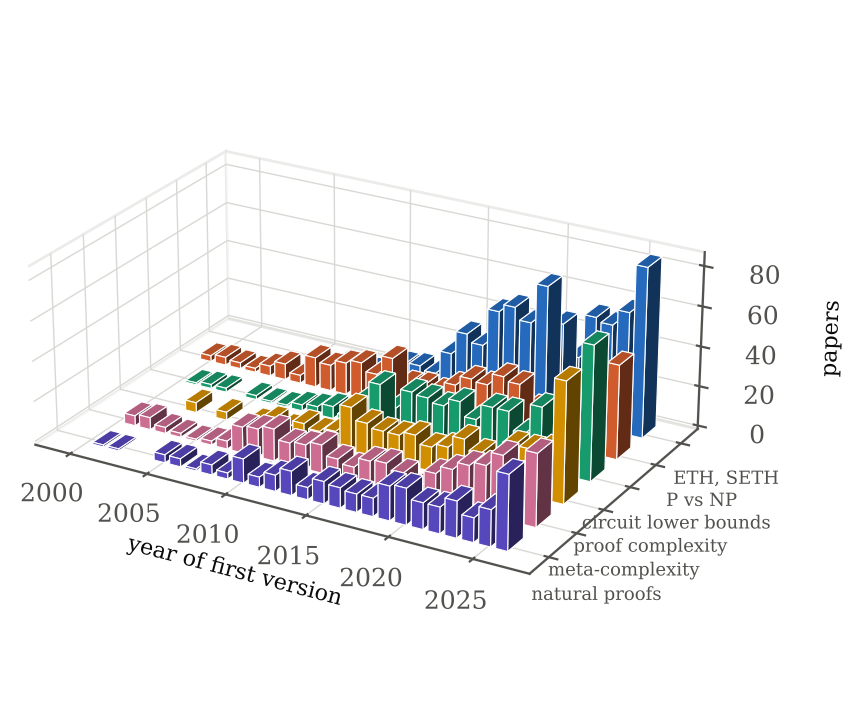
\includegraphics[width=0.95\textwidth]{fig_catalogue.png}
\caption{Papers of the arXiv catalogue in the core categories, by year of first
version and by topic (2,617 papers; a paper matching several topics is counted
once for each).}\label{fig:catalogue}
\end{figure}

\subsection{Where the problem stands}
No proof that $\Pc\ne\NP$ is known, and no known method is expected to give
one without new ideas, since each of the three barriers excludes a family of
techniques. The strongest explicit lower bounds for unrestricted circuits are
linear for functions in $\NP$ and, since \cite{OAI26}, of order $n\sqrt{\log
n}$ for a function in $\ENP$. Part~II extends the latter bound to circuits of
threshold, modular, symmetric and large table gates.

\part{New results}

%%==================================================================
\section{Circuits and tensor networks}\label{sec:networks}
%%==================================================================

\subsection{The circuit classes}
\begin{definition}\label{def:gates}
A \emph{circuit} $C$ with $m$ inputs consists of input variables
$x_1,\dots,x_m$ and gates $g_1,\dots,g_G$. Each gate $g$ has an ordered list of
$f(g)\ge0$ predecessors, each an input or an earlier gate, and one gate is the
output. The \emph{wires} of $C$ are the pairs (predecessor, gate), counted with
multiplicity, so their number is $\wires(C)=\sum_gf(g)$, and $s(C)=m+\wires(C)$.
For integers $F,\beta\ge1$ the class $\cK(F,\beta)$ consists of the circuits in
which every gate $g$, with inputs $y=(y_1,\dots,y_f)$, is of one of the
following kinds.
\begin{enumerate}[label=\textup{(\alph*)},leftmargin=2.2em]
\item \emph{Table gate}: $f\le F$, and $g(y)=\tau(y)$ for a function
$\tau:\{0,1\}^f\to\{0,1\}$ given by its truth table of $2^f$ bits.
\item \emph{Weighted gate}: integers $w_1,\dots,w_f$ with $|w_i|\le2^\beta$ are
given, $v(y)=\sum_iw_iy_i$, and $g(y)=\varphi(v(y))$, where $\varphi$ is one of
\[
[v\ge\theta],\qquad [v=\theta],\qquad [v\equiv\theta\bmod\mu]\ \ (1\le\mu\le2^\beta),
\]
for a given integer $\theta$, or, when $w_1=\dots=w_f=1$, an arbitrary function
$\varphi:\{0,\dots,f\}\to\{0,1\}$ given by its table of $f+1$ bits.
\end{enumerate}
The \emph{description} of $C$ lists $m$, the gates in order with their kinds,
predecessor lists, tables, weights, thresholds and moduli in binary, and the
output gate; $L$ denotes its length.
\end{definition}

A threshold $\theta$ outside $[-f2^\beta,f2^\beta+1]$ can be replaced by the
nearest end of this interval without changing the gate, and $\theta$ in a
congruence can be reduced modulo $\mu$, so we may and do assume that all
numbers in a description have $O(\beta+\log f)$ bits. A table gate of fan-in
zero is a constant.

\begin{example}\label{ex:gates}
Every gate of fan-in at most two is a table gate. An AND or OR of any fan-in is
the exact gate $[\sum_iy_i=f]$ or the threshold $[\sum_iy_i\ge1]$; a negation
is $[{-y_1}\ge0]$; parity and $\mathrm{MOD}_\mu$ gates are congruences; majority
and every symmetric function are unit-weight gates with a table on
$\{0,\dots,f\}$. A linear threshold function whose minimal integer weights
exceed $2^\beta$ is not a weighted gate of $\cK(F,\beta)$, but it is a table gate
when $f\le F$.
\end{example}

\subsection{Tensor networks}
We use the definitions of \cite[Section D.1]{OAI26}. A \emph{Boolean tensor
network} over a commutative ring $R$ is a finite multigraph $\mathcal G$ in
which every edge carries one bit. Each vertex $v$ has an ordered list $\delta(v)$
of incident edges, its \emph{ports}, and a tensor $T_v:\{0,1\}^{\delta(v)}\to R$.
Parallel edges occupy distinct ports. The \emph{contraction} of the network is
\[
Z=\sum_{x\in\{0,1\}^{E(\mathcal G)}}\ \prod_{v\in V(\mathcal G)}T_v\bigl(x|_{\delta(v)}\bigr).
\]
The size of the network is its number of edges, and the network is
\emph{bipartite} if $\mathcal G$ is. For integers $P_0,\ell\ge1$ put
$B_{P_0,\ell}=(\Z/2^{P_0}\Z)[V]/(V^\ell)$.

\begin{theorem}[\oai{}, {\cite[Theorem D.1]{OAI26}}]\label{thm:contraction}
Fix positive constants $C,A,b$. Let $s\ge2$ be an integer and let $L$ be the
total length of the graph and tensor descriptions of a bipartite tensor network
with at most $Cs$ edges, maximum degree at most $\lceil s^{9/10}\rceil$, and a
number of vertices bounded by a fixed polynomial in $s$, whose entries lie in
$B_{P_0,\ell}$ with $1\le P_0,\ell\le Cs$. Suppose that every entry can be
computed from the description in time $(s+L)^b2^{As^{9/10}}$ and space
$(s+L)^b$. Then the contraction can be computed deterministically in time
$(s+L)^{O(1)}2^{O(s/\sqrt{\log s})}$ and space $(s+L)^{O(1)}$, with constants
depending only on $C,A,b$.
\end{theorem}

The proof is reproduced in Appendix~\ref{app:contraction}. We use only the case
$\ell=1$, in which $B_{P_0,1}=\Z/2^{P_0}\Z$.

\begin{figure}[t]
\centering
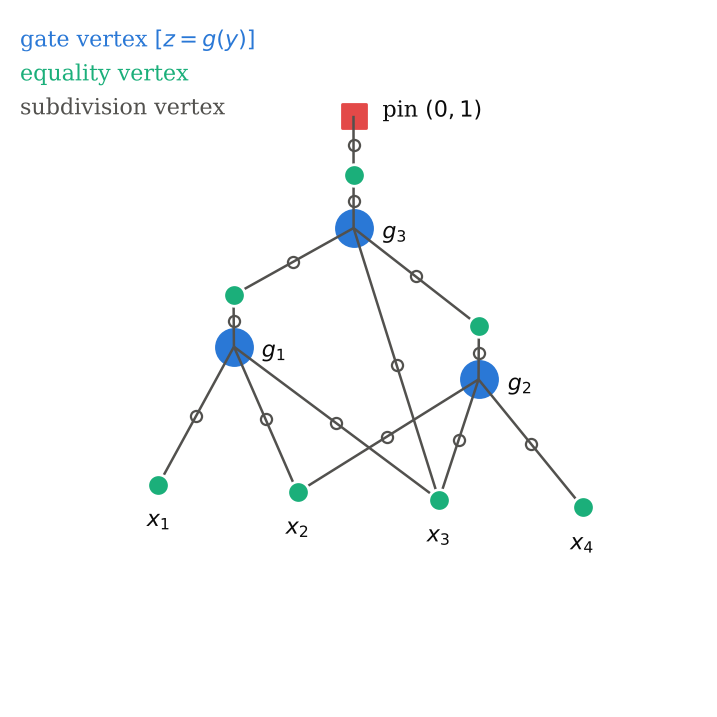
\includegraphics[width=0.66\textwidth]{fig_network.png}
\caption{The network of a small circuit (Section~\ref{sec:counting}). Gate
vertices (blue) carry the tables $[z=g(y)]$; each signal is distributed to its
ports by a tree of equality vertices (green), here a single vertex; a pin $(0,1)$ sits on the output;
every edge is then subdivided by a binary equality vertex (white), which makes
the network bipartite.}\label{fig:network}
\end{figure}

%%==================================================================
\section{Counting satisfying inputs}\label{sec:counting}
%%==================================================================

\begin{theorem}\label{thm:counting}
There are absolute constants $A_0,b_0$ and a deterministic algorithm that,
given the description of length $L$ of a circuit $C\in\cK(s^{4/5},s^{2/3})$ with
$s=s(C)\ge2$, computes $\#C=|\{x\in\{0,1\}^m:C(x)=1\}|$ in time
$(s+L)^{b_0}2^{A_0s/\sqrt{\log s}}$ and space $(s+L)^{b_0}$.
\end{theorem}

Here and below $s^{4/5}$ and $s^{2/3}$ stand for their integer parts. Since a
table gate has at most $s^{4/5}$ inputs, $L\le s^{O(1)}2^{s^{4/5}}$, and the time
is $2^{O(s/\sqrt{\log s})}$. The proof occupies the rest of this section.

\subsection{Normalisation}
A gate from which the output cannot be reached may be deleted; this removes its
wires and does not change the function. Constant gates of the same value may
be merged, which leaves the wires unchanged. We therefore assume that every
gate reaches the output and that there are at most two constant gates. Every
other gate has a wire, so
\begin{equation}\label{eq:gates}
G\le\wires(C)+2.
\end{equation}
Let $u$ be the number of inputs that are predecessors of no gate and that are
not the output. Then $\#C=2^u\,\#C'$, where $C'$ is $C$ with those inputs
removed, and $s(C')\le s(C)$. We assume $u=0$ from now on, restoring the factor
at the end.

\subsection{The network $\cN(C)$}
Put $K=\lfloor s^{4/5}\rfloor$, $\beta=\lfloor s^{2/3}\rfloor$ and
$b=\beta+\lceil\log K\rceil+2$. A gate is \emph{small} if it is a table gate or a
weighted gate of fan-in at most $K$, and \emph{big} otherwise. A \emph{signal}
is an input or a gate. For a signal $\sigma$ let $d_\sigma$ be its number of
\emph{occurrences}: one for its own value if $\sigma$ is a gate, one for each
wire leaving it, and one more if it is the output.

\smallskip\noindent\emph{Gate vertices.} A small gate $g$ with inputs
$y_1,\dots,y_f$ becomes a vertex $v_g$ with $f+1$ ports $(y_1,\dots,y_f,z)$ and
tensor $T(y,z)=[z=g(y)]$.

\smallskip\noindent\emph{Blocks.} A big weighted gate $g$ of fan-in $f>K$ has its
inputs split, in order, into $k=\lceil f/K\rceil$ blocks $I_1,\dots,I_k$ of at most
$K$ inputs each. For each block there is a vertex $v_{g,j}$ with ports
$(y_i)_{i\in I_j}$ and $b$ further ports $e_j=(e_{j,1},\dots,e_{j,b})$, and tensor
\[
T(y,e_j)=\bigl[\,\mathrm{val}(e_j)=P_j(y)+K2^\beta\,\bigr],\qquad
P_j(y)=\sum_{i\in I_j}w_iy_i,
\]
where $\mathrm{val}(e)=\sum_te_t2^{t-1}$. Since $|P_j|\le K2^\beta$, the integer
$P_j+K2^\beta$ lies in $[0,2K2^\beta]$ and has a unique binary expansion with
$b$ bits. A root vertex $r_g$ has the $kb$ ports $e_1,\dots,e_k$ and one port $z$,
with tensor
\[
T(e_1,\dots,e_k,z)=\Bigl[\,z=\varphi\Bigl(\sum_{j=1}^k\bigl(\mathrm{val}(e_j)-K2^\beta\bigr)\Bigr)\Bigr].
\]
The ports $e_j$ of $v_{g,j}$ and of $r_g$ are joined by $b$ edges, bit by bit.
For a big gate, the occurrence of a wire into $g$ is the corresponding input
port of a block vertex, and the occurrence of the value of $g$ is the port $z$
of the root.

\smallskip\noindent\emph{Equality trees and the pin.} Every occurrence of a
signal is a port of some vertex: an input port $y_i$ for a wire, the port $z$
for the value of a gate, and, for the output, the single port of a pin vertex
with tensor $(T(0),T(1))=(0,1)$. The $d_\sigma$ occurrences of $\sigma$ are
joined by an equality tree $Q_\sigma$: for $d_\sigma=1$ one edge to a vertex with
unary tensor $(1,1)$; for $d_\sigma=2$ two edges to a vertex with tensor $[a=a']$;
for $d_\sigma\ge3$ a tree with $d_\sigma$ leaf edges and $d_\sigma-2$ internal
vertices of degree three, each with tensor $[a=a'=a'']$. In every case each
common value on the leaf edges extends to exactly one assignment of the internal
edges with all tensors equal to one, and every other assignment has product
zero.

\smallskip\noindent\emph{Subdivision.} Finally every edge is subdivided once by a
vertex of degree two with tensor $[a=a']$. The vertices present before
subdivision form one side and the subdivision vertices the other, so $\cN(C)$
is bipartite. All entries are $0$ or $1$, read in $\Z/2^{m+1}\Z$.

Figures~\ref{fig:network} and~\ref{fig:blocks} show the construction.

\begin{figure}[t]
\centering
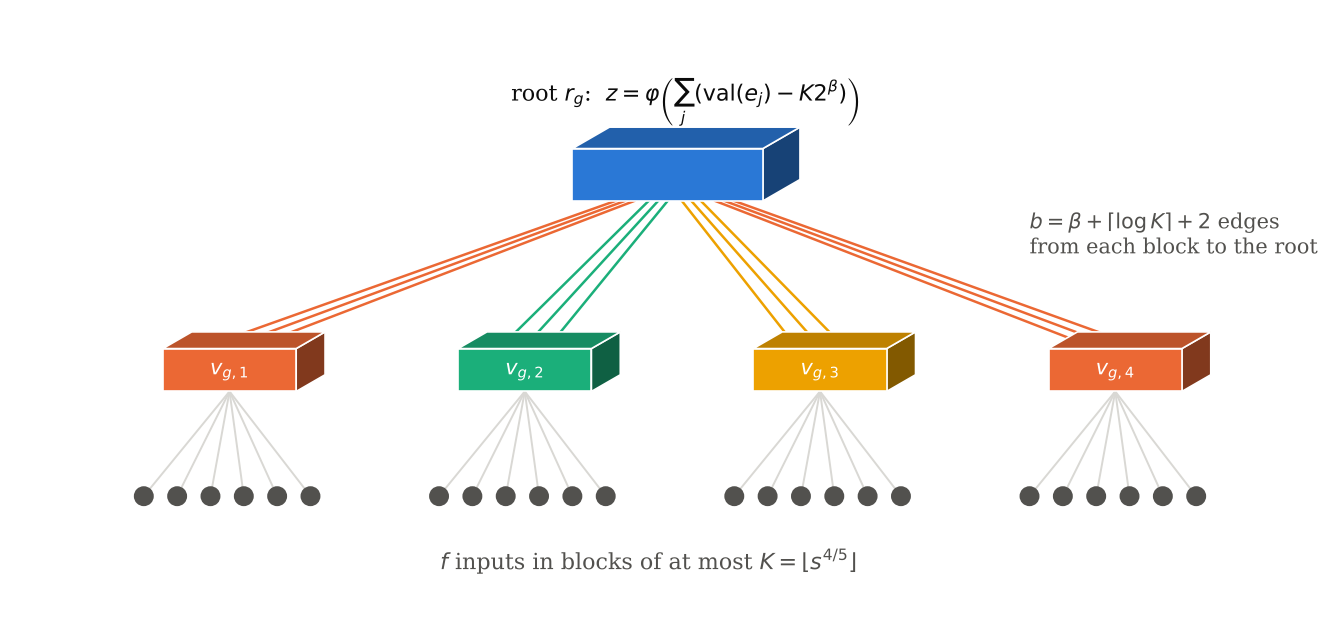
\includegraphics[width=0.92\textwidth]{fig_blocks.png}
\caption{A big weighted gate. Its $f$ inputs are cut into blocks of at most $K$
inputs; the block vertex $v_{g,j}$ writes the shifted partial sum
$P_j+K2^\beta$ on $b$ edges, and the root $r_g$ adds the decoded values and
applies $\varphi$. Every vertex then has degree $O(s^{13/15})$.}\label{fig:blocks}
\end{figure}

\begin{lemma}[Correctness]\label{lem:correct}
The contraction of $\cN(C)$ equals $\#C$ as an integer, and hence modulo
$2^{m+1}$.
\end{lemma}

\begin{proof}
Fix an assignment of the edges whose product of tensors is nonzero. The
subdivision vertices force both halves of each original edge to carry the same
bit. Each equality tree forces all occurrences of a signal $\sigma$ to carry a
common bit $a_\sigma$. At a small gate, $a_g=g(a_{\mathrm{pred}})$. At a big gate
the block tensors force $\mathrm{val}(e_j)=P_j(a)+K2^\beta$, so the sum read by
the root is $\sum_jP_j(a)=v(a)$ and $a_g=\varphi(v(a))$. The pin forces
$a_{\mathrm{out}}=1$. Conversely, an input $x$ with $C(x)=1$ determines the values
of all gates, hence all bits on all edges, and the product of the tensors at
that assignment is one. Distinct inputs give distinct assignments, and an input
with $C(x)=0$ gives none, because the pin would read zero. Since $u=0$, every
input occurs somewhere, so the nonzero terms are in bijection with the
satisfying inputs, and each is one.
\end{proof}

\begin{lemma}[Size]\label{lem:size}
For all $s$ larger than an absolute constant, $\cN(C)$ has at most $22s$ edges,
maximum degree at most $\lceil s^{9/10}\rceil$, and $O(s)$ vertices, and every
entry can be computed from the description of $C$ in time $(s+L)^{O(1)}$.
\end{lemma}

\begin{proof}
Let $W=\wires(C)$. The equality tree of $\sigma$ has at most $2d_\sigma$ edges, and
\[
\sum_\sigma d_\sigma=G+W+1,
\]
since each gate value, each wire and the output contribute one occurrence. A big
gate of fan-in $f$ has $k\le2f/K$ blocks and so $kb\le2fb/K$ edges between its
blocks and its root, and $b\le K$ for large $s$. Before subdivision the number
of edges is therefore at most $2(G+W+1)+2W\le6W+6\le11s$, using
\eqref{eq:gates} and $s\ge W$, $s\ge2$; subdivision doubles it. The number of
vertices is at most the number of edges plus the number of pins and unary
vertices, so it is $O(s)$.

Subdivision vertices have degree two and equality vertices degree at most
three. A small gate has degree $f+1\le K+1$, a block vertex at most $K+b$, and a
root
\[
kb+1\le\Bigl(\frac{s}{K}+1\Bigr)\bigl(s^{2/3}+\log s+3\bigr)+1=O(s^{1/5+2/3})=O(s^{13/15}).
\]
All of these are below $s^{9/10}$ for large $s$. An entry is a comparison of a
gate value with a table entry, a weighted sum of at most $s$ terms of $O(\beta+
\log s)$ bits, a binary expansion or a test of $\varphi$; each takes time
polynomial in $s+L$.
\end{proof}

\begin{proof}[Proof of Theorem~\ref{thm:counting}]
If $s$ is below the constant of Lemma~\ref{lem:size}, enumerate the $2^m$ inputs.
Otherwise normalise $C$, build $\cN(C)$ with its description of length
$(s+L)^{O(1)}$, and apply Theorem~\ref{thm:contraction} with $C=22$,
$P_0=m+1\le s$, $\ell=1$, any $A>0$ and the polynomial of Lemma~\ref{lem:size}.
By Lemma~\ref{lem:correct} the result is $\#C'\bmod2^{m+1}$. Multiply by $2^u$
modulo $2^{m+1}$; since $0\le\#C\le2^m$, the least nonnegative residue is $\#C$.
The bounds are those of Theorem~\ref{thm:contraction}.
\end{proof}

\begin{remark}\label{rem:space}
The algorithm uses space $(s+L)^{O(1)}$. A multitape Turing machine therefore
simulates it with a factor $(s+L)^{O(1)}$ in time, by scanning its workspace at
each access; this is the form used in Section~\ref{sec:lower}.
\end{remark}

\begin{corollary}\label{cor:classes}
For circuits whose gates are any mixture of gates of fan-in two, AND, OR and
parity gates of any fan-in, $\mathrm{MOD}_\mu$ gates with $\mu\le2^{s^{2/3}}$,
symmetric gates, and threshold gates with weights below $2^{s^{2/3}}$, the
number of satisfying inputs can be computed in time $L^{O(1)}2^{O(s/\sqrt{\log
s})}$, where $s$ is the number of inputs plus wires.
\end{corollary}

\begin{proof}
These circuits lie in $\cK(2,s^{2/3})$ by Example~\ref{ex:gates}, and here
$L=s^{O(1)}$ up to the bits of the weights, which are counted in $L$.
\end{proof}

%%==================================================================
\section{Zero-one programs}\label{sec:ilp}
%%==================================================================

\begin{corollary}[Theorem C]\label{cor:ilp}
Let $A\in\Z^{r\times n}$, $b\in\Z^r$ and $c\in\Z^n$, and put $\sigma=n+\nu(A)$,
where $\nu(A)$ is the number of nonzero entries of $A$. Suppose that every
entry of $A$ and $c$ has absolute value at most $2^{\sigma^{2/3}}$, and let $L$ be
the length of the input. Then, deterministically in time
$L^{O(1)}2^{O(\sigma/\sqrt{\log\sigma})}$ and polynomial space, one can
\begin{enumerate}[label=\textup{(\roman*)},leftmargin=2.2em]
\item compute the number of $x\in\{0,1\}^n$ with $Ax\le b$;
\item decide whether such $x$ exists and, if so, compute $\max\{c\cdot x:Ax\le
b,\ x\in\{0,1\}^n\}$ and a point attaining it.
\end{enumerate}
\end{corollary}

\begin{proof}
A row with no nonzero entry is the constant condition $0\le b_j$; if one fails,
the answer is zero, and otherwise drop it. So every row has a nonzero entry and
$r\le\nu(A)$. Row $j$ becomes the weighted gate
$h_j=[\sum_k(-a_{jk})x_k\ge-b_j]$, with $\nu_j$ wires, and their conjunction is the
exact gate $[\sum_jh_j=r]$ with $r$ wires. The circuit has $s=n+\nu(A)+r\le2\sigma$
and weights at most $2^{\sigma^{2/3}}\le2^{s^{2/3}}$, so it lies in
$\cK(2,s^{2/3})$ and Theorem~\ref{thm:counting} gives (i).

For (ii) add the gate $[c\cdot x\ge t]$, with $n$ wires, to the conjunction; the
circuit now has $s\le3\sigma$, and its weights are still at most
$2^{s^{2/3}}$. The value $\max c\cdot x$ lies in $[-n2^{\sigma^{2/3}},
n2^{\sigma^{2/3}}]$, so binary search over $t$ finds it with
$O(\sigma^{2/3}+\log n)$ counting calls. A maximiser is found by fixing
$x_1,x_2,\dots$ in turn, replacing $b$ by $b-a_kx_k$ and keeping a value for which
the count with $c\cdot x\ge t_{\max}$ stays positive; this uses $n$ further calls,
each on a smaller program. The calls are made one after another, so the space
stays polynomial.
\end{proof}

When $\nu(A)=O(n)$ the bound is $2^{O(n/\sqrt{\log n})}$. Problems with $O(n)$
constraints of bounded support, such as exact cover by sets of bounded size or
knapsack with conflict constraints along the edges of a sparse graph, are of
this form, with weights of up to $\sigma^{2/3}$ bits in the knapsack row.

%%==================================================================
\section{The lower bound}\label{sec:lower}
%%==================================================================

The argument is that of \cite[Appendix C.1]{OAI26}, itself an instance of
Williams' method \cite{Wil13}; what changes is the circuit class, which is
handled by Theorem~\ref{thm:counting} in place of the $3$-CNF algorithm.

\subsection{Ingredients}
All machines are multitape Turing machines. We use three known results.

\begin{lemma}[Nondeterministic hierarchy, {\cite{Zak83}}; see {\cite[Theorem 2.1]{Wil13}}]\label{lem:zak}
There is a unary language $H\subseteq\{1\}^*$ with
$H\in\NTIME(2^n)\setminus\NTIME(2^{n/2})$.
\end{lemma}

\begin{lemma}[Local reduction, {\cite[Theorem 1 and Section 6]{JMV15}}]\label{lem:jmv}
Let $M$ be the machine deciding $H$ in time $2^n$. There are $q=n+O(\log n)$,
$v=n+O(\log n)$, a fixed integer $w$, and a deterministic polynomial-time
algorithm that, given $n$, outputs a map
\[
D_n:\{0,1\}^q\to\bigl(\{0,1\}^v\bigr)^3\times\{0,1\}^3
\]
with the following properties. Let $\varphi_n$ be the $3$-CNF on the variables
$\{X_\lambda:\lambda\in\{0,1\}^v\}$ whose clauses are, for $i\in\{0,1\}^q$ with
$D_n(i)=(\lambda_1,\lambda_2,\lambda_3,\epsilon_1,\epsilon_2,\epsilon_3)$, the
clauses $X_{\lambda_1}^{\epsilon_1}\vee X_{\lambda_2}^{\epsilon_2}\vee
X_{\lambda_3}^{\epsilon_3}$, where $X^1=X$ and $X^0=\neg X$. Then $\varphi_n$ is
satisfiable if and only if $1^n\in H$, and each output bit of $D_n$ depends on at
most $w$ bits of $i$.
\end{lemma}

The reduction of \cite{JMV15} applies to any nondeterministic computation of
length $T$, here $T=2^nn^{O(1)}$ including the overhead of the simulation, and
gives $\log T+O(\log\log T)$ index bits and clause bits computable by decision
trees of constant depth.

\begin{lemma}[Decoder circuits]\label{lem:decoder}
There is a circuit $\Delta_n$ that computes $D_n$, consists of $O(n)$ table
gates of fan-in at most $w$, and is constructed in time polynomial in $n$.
\end{lemma}

\begin{proof}
This is the argument of \cite[Appendix C.1]{OAI26}. For an output bit $o$ of
$D_n$, evaluate $D_n$ at the zero string and at all strings of Hamming weight
at most $w$; this is polynomially many evaluations since $w$ is fixed. If $o$
depends on coordinate $c$, there are two strings that differ only in $c$ and
give different values of $o$; setting to zero all coordinates outside the
support of $o$ keeps the values, so two such strings of weight at most $w$
exist and are among those evaluated. Hence the evaluations recover the support
of $o$ and its truth table on it. Each output bit is then one table gate of
fan-in at most $w$, and $D_n$ has $O(n)$ output bits.
\end{proof}

\subsection{The language $\Wl$}
Fix an integer $d\ge1$ with $v\le dn$ for all large $n$; $d=2$ will do. For a
label $\lambda\in\{0,1\}^v$ write $\bar\lambda\in\{0,1\}^{dn}$ for $\lambda$
followed by $dn-v$ zeros, and regard $\varphi_n$ as a formula on all $2^{dn}$
variables $X_{\bar\lambda}$, most of which do not occur. For $|i|=dn$, define
$\Wl(i)$ as bit $i$ of the lexicographically first satisfying assignment of
$\varphi_n$, with variables ordered by their labels, when $\varphi_n$ is
satisfiable, and $\Wl(i)=0$ otherwise; for lengths not divisible by $d$ put
$\Wl(i)=0$.

\begin{lemma}\label{lem:WinENP}
$\Wl\in\ENP$.
\end{lemma}

\begin{proof}
On an input of length $N=dn$, write out the $2^q$ clauses of $\varphi_n$ by
evaluating $D_n$, in time $2^{O(n)}$. Ask the oracle whether $\varphi_n$ is
satisfiable. If it is, determine the first assignment bit by bit: having fixed
a prefix, ask whether $\varphi_n$ with the prefix followed by zero has a
satisfying extension, and append zero or one accordingly. The queries have
length $2^{O(n)}$, and at most $2^{dn}$ of them determine bit $i$. The time is
$2^{O(N)}$.
\end{proof}

\subsection{From counting to wires}
\begin{theorem}[Transfer; Theorem D]\label{thm:transfer}
Let $\gamma>0$ be rational, let $A_1,b_1>0$, and suppose that a deterministic multitape Turing
machine decides, for every circuit $C\in\cK(s^{4/5},s^{2/3})$ with $s=s(C)\ge2$
given by a description of length $L$, whether $C$ is satisfiable, in time
$(s+L)^{b_1}2^{A_1s/(\log s)^\gamma}$. Then there is $c>0$ such that for infinitely
many $N$, every circuit in $\cK(N^{3/4},N^{1/2})$ with $N$ inputs deciding $\Wl$ on
$\{0,1\}^N$ has more than $cN(\log N)^\gamma$ wires.
\end{theorem}

\begin{proof}
Fix a rational $\eta$ with $0<\eta<1/(12A_1)$ and put
$s_n=\lfloor\eta n\lfloor\lfloor\log n\rfloor^\gamma\rfloor\rfloor$, which is
computable in time polynomial in $\log n$. Suppose,
for contradiction, that for all large $n$ some circuit $E_n\in\cK((dn)^{3/4},
(dn)^{1/2})$ with $dn$ inputs and at most $s_n$ wires decides $\Wl$ on
$\{0,1\}^{dn}$. We decide $H$ as follows. Reject inputs that are not unary. On
$1^n$, guess a circuit $E$ in this class with at most $s_n$ wires; its
description has length $L_E=2^{O(n^{3/4})}$, since it has at most $s_n$ gates,
each with a table of at most $2^{(dn)^{3/4}}$ bits or $O(s_n)$ numbers of
$O(\sqrt n)$ bits. Build the test circuit $\mathcal T$ with inputs
$i\in\{0,1\}^q$:
\begin{enumerate}[label=\textup{(\arabic*)},leftmargin=2em]
\item the decoder $\Delta_n$ of Lemma~\ref{lem:decoder} computes
$(\lambda_1,\lambda_2,\lambda_3,\epsilon_1,\epsilon_2,\epsilon_3)$;
\item three copies of $E$ read $\bar\lambda_1,\bar\lambda_2,\bar\lambda_3$, the
padding zeros coming from one constant gate;
\item one table gate of fan-in six outputs one if and only if every literal
$E(\bar\lambda_t)^{\epsilon_t}$ is false, that is, if the clause of index $i$ is
violated by the assignment $\lambda\mapsto E(\bar\lambda)$.
\end{enumerate}
Accept if and only if $\mathcal T$ is unsatisfiable.

If $1^n\in H$, then $\varphi_n$ is satisfiable and the guess $E=E_n$ computes a
satisfying assignment, so no clause is violated and the machine accepts. If
$1^n\notin H$, then every $E$ defines an assignment that violates some clause of
$\varphi_n$, so $\mathcal T$ is satisfiable and the machine rejects. Thus the
machine decides $H$.

The circuit $\mathcal T$ has $q=n+O(\log n)$ inputs and at most
$3s_n+O(n)$ wires, so $n\le s(\mathcal T)\le3s_n+B n$ for a constant $B$. Its
table gates have fan-in at most $\max(w,6,(dn)^{3/4})$ and its weights at most
$2^{(dn)^{1/2}}$. For $n\ge d^{15}$ we have $(dn)^{3/4}\le n^{4/5}$, and for
$n\ge d^3$ we have $(dn)^{1/2}\le n^{2/3}$; since $s(\mathcal T)\ge n$, the
circuit lies in $\cK(s^{4/5},s^{2/3})$ with $s=s(\mathcal T)$ for all large $n$.
By hypothesis its satisfiability is decided in time
\[
(s+L)^{b_1}2^{A_1s/(\log s)^\gamma}
\le2^{O(n^{3/4})}\cdot2^{A_1(3s_n+Bn)/(\log n)^\gamma}
=2^{(3A_1\eta+o(1))n},
\]
and $3A_1\eta<1/4$. Guessing $E$ and building $\mathcal T$ take
$2^{O(n^{3/4})}$ steps. Hence $H\in\NTIME(2^{n/2})$ after hardwiring finitely
many lengths, which contradicts Lemma~\ref{lem:zak}.

Therefore, for infinitely many $n$, every circuit in
$\cK((dn)^{3/4},(dn)^{1/2})$ deciding $\Wl$ on length $N=dn$ has more than $s_n$
wires. Since $\log n=\log N-\log d$, we have $s_n\ge(\eta/d)(1-o(1))N(\log
N)^\gamma$, and $c=\eta/(2d)$ works.
\end{proof}

\begin{theorem}[Theorem B]\label{thm:lower}
There are a language $\Wl\in\ENP$ and a constant $c>0$ such that for infinitely
many $N$ every circuit in $\cK(N^{3/4},N^{1/2})$ with $N$ inputs that decides
$\Wl$ on $\{0,1\}^N$ has more than $cN\sqrt{\log N}$ wires.
\end{theorem}

\begin{proof}
Theorem~\ref{thm:counting} with Remark~\ref{rem:space} decides satisfiability
by testing whether $\#C>0$ on a multitape machine in time
$(s+L)^{b_0+O(1)}2^{A_0s/\sqrt{\log s}}$. Apply Theorem~\ref{thm:transfer} with
$\gamma=\tfrac12$, and Lemma~\ref{lem:WinENP}.
\end{proof}

\begin{corollary}\label{cor:lowerclasses}
For infinitely many $N$, the language $\Wl$ on $\{0,1\}^N$ is not decided by any
circuit with fewer than $cN\sqrt{\log N}$ wires whose gates are gates of fan-in
two, AND, OR, parity, $\mathrm{MOD}_\mu$ and symmetric gates of any fan-in, and
threshold gates with weights below $2^{\sqrt N}$, in any combination and at any
depth.
\end{corollary}

\begin{proof}
Such circuits lie in $\cK(2,N^{1/2})\subseteq\cK(N^{3/4},N^{1/2})$ by
Example~\ref{ex:gates}.
\end{proof}

\subsection{Comparison}
For fan-in-two circuits, Theorem~B is \cite[Corollary 1.4]{OAI26}, since $g$
such gates use at most $2g$ wires. For threshold circuits, the bounds of
\cite{IPS97,KW16,CSS18} hold for functions in $\Pc$ and are stronger at each
fixed depth, but they tend to linear as the depth grows; Theorem~B is weaker at
small depth and holds at every depth. To the author's knowledge no superlinear
lower bound for a language in $\ENP$ against unbounded-depth circuits of
threshold or $\mathrm{MOD}_\mu$ gates, or of arbitrary gates of fan-in
$N^{3/4}$, was known before.

%%==================================================================
\section{Limits of the method}\label{sec:limits}
%%==================================================================

\subsection{The exponent $\sqrt{\log N}$}
Theorem~\ref{thm:transfer} converts a saving of $(\log s)^\gamma$ in the exponent
of a satisfiability algorithm into a factor $(\log N)^\gamma$ in the lower bound,
and conversely the method can give no more: the test circuit has $\Theta(s_n)$
wires and must be checked in time $2^{n/2}$. In the proof of
Theorem~\ref{thm:contraction} the factor $\sqrt{\log s}$ has a definite source
(Appendix~\ref{app:modes}). At a call with $M$ wires, an interpolation node of
two-adic level $i$ has about $M/D$ mode variables of each weight, $D=L/2^i$,
and works at a precision of order $MD/u$, where $u$ is the number of retained
levels; the number of admissible mode monomials is then
$\exp(O(\sqrt{M\cdot MD/u\cdot D^{-1}}))=\exp(O(M/\sqrt u))$. The number of
levels is at most $\log L$, and the packet length $L$ must stay below a small
power of $s$, because a packet tensor costs $\exp(O(L\log s))$ to evaluate.
So $u=O(\log s)$, and the recursion, which divides $M$ by eight at each depth,
sums these exponents to $O(s/\sqrt{\log s})$. A bound $cN\log N$ would need a contraction algorithm
whose exponent is $O(s/\log s)$, and the present design does not give one.

\subsection{Fan-in and weights}
Some restriction on the table gates is unavoidable, since one gate of fan-in
$N$ decides any language. In the proof, a table gate of fan-in $F$ costs $2^F$ in
the guess and in the entries of the network, and Theorem~\ref{thm:contraction}
tolerates entry costs of $2^{O(s^{9/10})}$; the exponents $4/5$, $2/3$ and $3/4$,
$1/2$ were chosen for simplicity and are not optimal. Weights enter through the
number $b$ of bits per block, which must keep the root degree below $s^{9/10}$.

\subsection{Superpolynomial bounds}
Williams' theorem \cite{Wil13} converts an algorithm for circuits of polynomial
size with $n$ inputs into a lower bound only if it beats $2^n$ by a
superpolynomial factor. Theorem~\ref{thm:counting} is measured in the size: for
a circuit with $n$ inputs and $n^k$ wires it gives time $2^{O(n^k/\sqrt{\log
n})}$, which is far above $2^n$. Superpolynomial lower bounds for $\ENP$, and a
fortiori for $\NP$, need algorithms whose running time depends on the number of
inputs; nothing in the tensor method provides this.

\subsection{From $\ENP$ to $\NP$}
The language $\Wl$ is defined by the first satisfying assignment of an
exponentially long formula and is computed with an $\NP$ oracle in exponential
time; it is not known to lie in $\NP$. The lower bound for
$\Wl$ therefore says nothing about $\Pc$ versus $\NP$ directly, and even a
superpolynomial lower bound for $\ENP$ would leave the question open, since
$\Pc\ne\NP$ is not implied by lower bounds for exponential-time classes.

\subsection{The barriers}
The proof diagonalises against $\NTIME(2^{n/2})$ through a single language, so
it is not a natural proof in the sense of \cite{RR97}. Because the table gates
may compute arbitrary functions of $N^{3/4}$ inputs, Theorem~B holds for circuits
with small gates of arbitrary function. The locality barrier \cite{CHOPRS22}
shows that the magnified statements of \cite{OS18} are false for circuits with
small oracle gates, so an argument that applies equally to such gates, as this
one does, is not expected to reach them. The barrier concerns techniques and
does not formally exclude any extension, but it indicates that the route from
Theorem~B to superpolynomial bounds does not pass through magnification.

\appendix

%%==================================================================
\section{Proof of the contraction theorem}\label{app:contraction}
%%==================================================================

This appendix gives the proof of Theorem~\ref{thm:contraction}. The argument
and its parameters are those of \oai{} \cite[Appendix D.4]{OAI26}; the
presentation follows theirs step by step, with some computations written out
in more detail. Throughout, $\log$ is to base two and $\ln$ is natural. A call
of the recursion receives a bipartite network with $M$ edges and a working
precision $p$, and returns its contraction modulo $2^p$. One side of the
network is called the row side and the other the column side; the ports of
row vertices are \emph{row ports} and those of column vertices \emph{column
ports}.

\subsection{The coefficient ring}\label{app:ring}
Put $\lambda=\lceil\log s\rceil$ and $e=4\lambda$. Choose a monic $f\in\Z[U]$ of
degree $e$ with coefficients in $\{0,1\}$ whose reduction modulo two is
irreducible; such $f$ exists because $\F_{2^e}$ exists, and it is found in time
polynomial in $s$ by testing the $2^e=s^{O(1)}$ candidates for divisibility by
every monic polynomial of degree at most $e/2$ over $\F_2$ \cite{vzGG13}. Put
\[
\cO=\Z_{(2)}[U]/(f),\qquad K=\Q[U]/(f),\qquad \cA=\cO[V]/(V^\ell),\qquad
\cA_p=\cA/(2^p),
\]
where $\Z_{(2)}$ is the ring of rationals with odd denominator. Since $f$ is
irreducible modulo two it is irreducible over $\Q$, so $K$ is a field. For
$x\in K^\times$ let $\vtwo(x)$ be the least two-adic valuation of its coordinates
in the basis $1,U,\dots,U^{e-1}$. Then $\cO/2\cO=\F_{2^e}$, and factoring out the
least coordinate valuation shows $\vtwo(xy)=\vtwo(x)+\vtwo(y)$. An element of
$\cO$ that is nonzero modulo two is a unit, since the determinant of its
multiplication matrix is odd. Arithmetic in $\cA_p$, with coordinates in the
bases $1,U,\dots,U^{e-1}$ and $1,V,\dots,V^{\ell-1}$ stored as residues in
$[0,2^p)$, takes time and space polynomial in $s,p,\ell$; units are inverted by
inversion modulo two and Newton lifting. Divisibility in $\cA$ is coordinatewise.

The lifts to $\cO$ of the $2^e\ge s^4$ elements of $\F_{2^e}$, taken with
coordinates in $\{0,1\}$, have pairwise differences that are units; Lagrange
interpolation at fewer than $s^4$ of them is therefore valid over every
$\cA_p$. The original entries lie in $B_{P_0,\ell}\subseteq\cA_{P_0}$, and the
contraction, a polynomial in the entries, is computed in $\cA_{P_0}$ and read off
in $B_{P_0,\ell}$.

When the precision grows, each tensor entry is lifted separately: an entry
specified modulo $2^{p_c}$ is replaced by the element of $\cA$ whose coordinates
are its integer representatives in $[0,2^{p_c})$. This lift is not additive, but
it is fixed: every tensor carries the precision $p_c$ at which it was created,
and every later evaluation uses the same representatives. Precisions strictly
increase along a recursive path, so the representatives are canonical at every
later precision.

\subsection{Parameters and packing}\label{app:packing}
All inequalities below hold for $s$ larger than a constant depending on
$C,A,b$; smaller sizes are handled by direct summation. Put
\[
H=\Bigl\lceil\frac{s}{\lfloor\sqrt\lambda\rfloor}\Bigr\rceil,\qquad r=64,\qquad
\varepsilon=\frac1{128\cdot1024},\qquad\Delta=\lceil s^{9/10}\rceil.
\]
A call with $M\le H$ edges is a \emph{leaf} and is evaluated by summing over
all $2^M$ edge assignments. At an \emph{active} call at depth $d$ (the root has
depth zero) put
\begin{equation}\label{eq:params}
u=u_d=\Bigl\lfloor\frac{\varepsilon\lambda}{2^d}\Bigr\rfloor,\qquad
a=a_d=2\sum_{j=0}^du_j,\qquad L=2^a,\qquad \Darr=r^{2a}.
\end{equation}
It will be shown that every child of a call with $M$ edges has at most $M/8$
edges and maximum degree at most $\Delta$. Hence on every active path
$H<M\le Cs8^{-d}$, so $8^d<C\lfloor\sqrt\lambda\rfloor+1$ and
$d\le\frac16\log\lambda+O(1)$. Consequently, on every active call,
\begin{equation}\label{eq:inv1}
u=\Theta(\lambda/2^d),\qquad \lambda^{4/5}\le u\le M,\qquad a\le4\varepsilon\lambda,
\qquad L,\Darr\le s^{1/1000},
\end{equation}
since $2^d=O(\lambda^{1/6})$, $a\le4u_0$ and $\Darr=2^{12a}\le2^{48\varepsilon\lambda}$.
In particular
\begin{equation}\label{eq:inv2}
M\ge2\Darr^2\Delta,\qquad M\ge L\Darr,\qquad 2L\le\Delta,
\end{equation}
because $M>H\ge s^{1-o(1)}$ while the right sides are $O(s^{9/10+1/500})$.

\begin{lemma}[Packing]\label{lem:packing}
Assume \eqref{eq:inv2}. One can label the vertices on each side by elements of
$[r]^a$ and place the edges into \emph{packets} of $L$ slots so that:
\begin{enumerate}[label=\textup{(\arabic*)},leftmargin=2.2em]
\item there are at most $3M/L$ packets, every edge occupies the same slot at its
row end and at its column end, and unused slots carry no ports;
\item in every packet and every coordinate $c\in[a]$ the unordered pair of row
and column symbols is fixed, and when the two symbols differ, bit $c$ of the
slot number records which of them is the row symbol;
\item for every coordinate and every symbol, at most $3M/r$ real ports on each
side belong to vertices with that symbol in that coordinate.
\end{enumerate}
The construction takes time and space polynomial in $s+L$.
\end{lemma}

\begin{proof}
The \emph{pair label} of an edge is the pair (row label, column label), one of
$\Darr$ values; let $X_\gamma$ be the number of edges with pair label $\gamma$.
For independent uniform labels,
\[
\mathbb E\sum_\gamma\Bigl(X_\gamma-\frac M{\Darr}\Bigr)^2
=\sum_{e,e'}\Bigl(\Pr[\gamma(e)=\gamma(e')]-\frac1{\Darr}\Bigr),
\]
the sum running over ordered pairs of edges. If $e$ and $e'$ have disjoint
endpoints their labels are independent and the term vanishes. At most $2M\Delta$
ordered pairs share an endpoint, and each term is at most one, so the
expectation is at most $2M\Delta$. Labelling the vertices one at a time and
choosing, among the $r^a$ labels of the next vertex, one that does not increase
the conditional expectation \cite{Rag88} gives a deterministic labelling with
the same bound; each conditional expectation is a sum over pairs of edges of
probabilities involving at most four vertices, so it is computed exactly in
polynomial time. Every load is then at most $M/\Darr+\sqrt{2M\Delta}$. Pad every
pair-label class to $H_{\mathrm{pad}}$ slots, the largest load rounded up to a
multiple of $L$; by \eqref{eq:inv2},
\[
H_{\mathrm{pad}}\le\frac M{\Darr}+\sqrt{2M\Delta}+L\le\frac{3M}{\Darr}.
\]
Group the pair labels by the unordered pair of symbols in each coordinate. If
$a'$ coordinates of a group have unequal symbols, the group consists of $2^{a'}$
pair labels, which differ in orientation. Form packets of $L$ slots by taking
$2^{a-a'}$ slots of each of these $2^{a'}$ labels; this is possible since
$H_{\mathrm{pad}}$ is divisible by $L$. Number the positions of a packet from $0$
to $L-1$ so that bit $c$ gives the orientation when the pair in coordinate $c$ is
unequal and indexes copies otherwise, with one convention throughout a packet.
There are $H_{\mathrm{pad}}\Darr/L\le3M/L$ packets. In a fixed coordinate a fixed
symbol is the row symbol of exactly $1/r$ of the padded pair labels, so it has at
most $H_{\mathrm{pad}}\Darr/r\le3M/r$ real row ports, and likewise for columns.
\end{proof}

\subsection{A Cauchy deformation}\label{app:cauchy}
Fix an active call, its packets and its lifted tensors. Put
\[
S=\{-L,-L+1,\dots,L-1\},\qquad C(T)=\prod_{t\in S}(T-t),\qquad \alpha=2^{a+1}.
\]
For a row slot $x$ and a column slot $y$ of the same packet put
\begin{equation}\label{eq:W}
W_{xy}(T)=\frac{C(T)}{C'(0)\,(T-(y-x))},
\end{equation}
a polynomial of degree $2L-1$ over $\Q$, since $y-x\in S$; entries between
different packets are zero, and $W$ is restricted to real ports. At $T=0$ the
diagonal entries are one and the others vanish, because $C(T)/T\to C'(0)$ and
every other quotient keeps the factor $T$; so $W(0)$ is the identification of
row and column ports given by the edges. Let $A(Y)$ be the product of the
lifted row tensors on a row assignment $Y\in\{0,1\}^M$ and $B(X)$ the product of
the lifted column tensors on a column assignment $X$. With $l_0(z)=1-z$ and
$l_1(z)=z$ put
\begin{equation}\label{eq:F}
F(T)=\sum_{X,Y\in\{0,1\}^M}A(Y)B(X)\prod_{\text{row ports }x}l_{Y_x}\bigl((W(T)X)_x\bigr).
\end{equation}
Its coefficients lie in $K[V]/(V^\ell)$, its degree is at most $M(2L-1)$, and,
since $\prod_xl_{Y_x}(X_x)=[Y=X]$, $F(0)=\sum_XA(X)B(X)$ is the contraction of the
lifted tensors.

\begin{lemma}[Integrality]\label{lem:integral}
For every $t\in S$ the entries of $W(t+\alpha z)$ lie in $\cO[z]$ and
$F(t+\alpha z)\in\cA[z]$. Given the coordinates of $\zeta$ modulo $2^p$, each
$W_{xy}(t+\alpha\zeta)\bmod2^p$ is computed in time polynomial in $s,p$.
\end{lemma}

\begin{proof}
$S$ is a complete residue system modulo $2^{a+1}$. For $q\ne t$ in $S$ one has
$\vtwo(t-q)\le a$, and the number of $q$ with $\vtwo(t-q)=k$ does not depend on
$t$; hence $\vtwo(C'(t))=\vtwo(C'(0))$. In
\[
\frac{C(t+\alpha z)}{C'(0)}=\frac{\alpha z\prod_{q\ne t}(t-q+\alpha z)}{C'(0)}
\]
each factor $t-q+\alpha z$ is divisible coefficientwise by $2^{\vtwo(t-q)}$, so
after cancelling these powers against the denominator the polynomial is
divisible by $2^{a+1}$. Formula~\eqref{eq:W} omits the factor indexed by
$q=t-(y-x)$. If $y-x=t$ the omitted factor is $\alpha z$ and the rest is
integral; otherwise $\alpha z$ remains, the omitted factor has content
$2^{\vtwo(t-y+x)}$ with $\vtwo(t-y+x)\le a$, and the quotient is still
integral. Substituting in \eqref{eq:F} gives the claim for $F$. To evaluate,
divide each factor $t-q+\alpha z$ by $2^{\vtwo(t-q)}$, cancel the remaining
powers of two against $C'(0)$, invert its odd part modulo $2^p$, and multiply
the $O(L)$ factors at $\zeta$.
\end{proof}

\subsection{Tapered Hermite recovery}\label{app:hermite}
\begin{lemma}[Recovery]\label{lem:recovery}
Let $1\le u\le a$ and $M\ge u$, and put $h=\lceil3M/u\rceil$. For $t\in S\setminus\{0\}$
let
\[
i=\vtwo(t),\qquad q_t=q(i)=h\max(0,u-i),\qquad D_t=L/2^i .
\]
Let $F\in(K[V]/(V^\ell))[T]$ have degree at most $M(2L-1)$, with $F(0)\in\cA$ and
$F(t+\alpha z)\in\cA[z]$ for all $t\in S$. Then $F(0)\bmod2^p$ is determined by,
and computable in polynomial time from, the first $q_t$ coefficients of
\[
F(t+\alpha z)\bmod2^{p_t},\qquad p_t=p+8hD_t+8M(a+1),
\]
for the $t$ with $q_t>0$.
\end{lemma}

\begin{proof}
There are $L$ odd points in $S$, each with $q_t=hu\ge3M$, so
$\sum_{t\ne0}q_t\ge3ML>M(2L-1)$; also $q_t\le hu\le4M$. For $t$ with $q_t>0$ put
\[
E_t(T)=\prod_{q\in S\setminus\{0,t\}}\Bigl(\frac{T-q}{t-q}\Bigr)^{q_q}.
\]
We claim
\begin{equation}\label{eq:hermite}
F(0)=\sum_{t:\,q_t>0}E_t(0)\,\Bigl[\frac{F(t+\alpha z)}{E_t(t+\alpha z)}\Bigr]_{<q_t}\Bigl(-\frac t\alpha\Bigr),
\end{equation}
where $[\cdot]_{<q}$ truncates a power series in $z$ below degree $q$. Replace $0$
by an indeterminate $T$ and $-t/\alpha$ by $(T-t)/\alpha$ on the right. The
summand of $t$ agrees with $F$ to order $q_t$ at $T=t$ and vanishes to order
$q_{t'}$ at every other node $t'$, and its degree is below $\sum q_t$. So the
difference with $F$ is divisible by $\prod_{t\ne0}(T-t)^{q_t}$ and has smaller
degree, hence vanishes; this is Hermite interpolation by the Chinese remainder
theorem \cite[Section 5.6]{vzGG13}.

Each factor of $E_t(t+\alpha z)$ is a power of $1+\alpha z/(t-q)$, which is
integral with constant term one, so the reciprocal truncated below $q_t$ is
integral and the quotient in \eqref{eq:hermite} loses no precision.

Fix $i=\vtwo(t)$ and $D=D_t$. Points $q$ with $\vtwo(q)<i$ have
$\vtwo(t-q)=\vtwo(q)$ and contribute nothing to $\vtwo(E_t(0))$. For $1\le j\le
a-i$ there are $D/2^j$ points with $\vtwo(q)=i+j$, for which $\vtwo(t-q)=i$, and
$D/2^j$ points with $\vtwo(t-q)=i+j$, for which $\vtwo(q)=i$; these exhaust the
points of valuation at least $i$ other than $t$, since the nonzero differences
have valuation at most $a$. Therefore
\begin{equation}\label{eq:vEt}
\vtwo(E_t(0))=\sum_{q\ne0,t}q_q\bigl(\vtwo(q)-\vtwo(t-q)\bigr)
=D\sum_{j=1}^{a-i}\frac j{2^j}\bigl(q(i+j)-q(i)\bigr)\ \ge\ -6Dh,
\end{equation}
because $q(i+j)-q(i)\ge-hj$ and $\sum_{j\ge1}j^2/2^j=6$. Evaluating a polynomial of
degree below $q_t\le4M$ at $-t/\alpha$, whose valuation is at least $-(a+1)$,
loses at most $4M(a+1)$ powers of two. Hence replacing each quotient coefficient
by any lift of its residue modulo $2^{p_t}$ changes the summand by an element of
$2^p\cA$, since $p_t-p>6Dh+4M(a+1)$. The multipliers $E_t(0)(-t/\alpha)^j$ are
rationals of polynomial bit length, so the combination is carried out exactly
with a common denominator, after which the powers of two are cancelled and the
result reduced modulo $2^p$.
\end{proof}

The tapering of the multiplicities is what makes the precision affordable. If
every level below $u$ received the same multiplicity $q_*=\Theta(M)$, the level
$i=u-1$ would lose $q_*D\sum_jj/2^j=\Theta(MD)$ powers of two in
\eqref{eq:vEt}; with multiplicities decreasing by $h=\Theta(M/u)$ per level the
loss is $O(MD/u)$.
Figure~\ref{fig:taper} compares the two choices.

\begin{figure}[t]
\centering
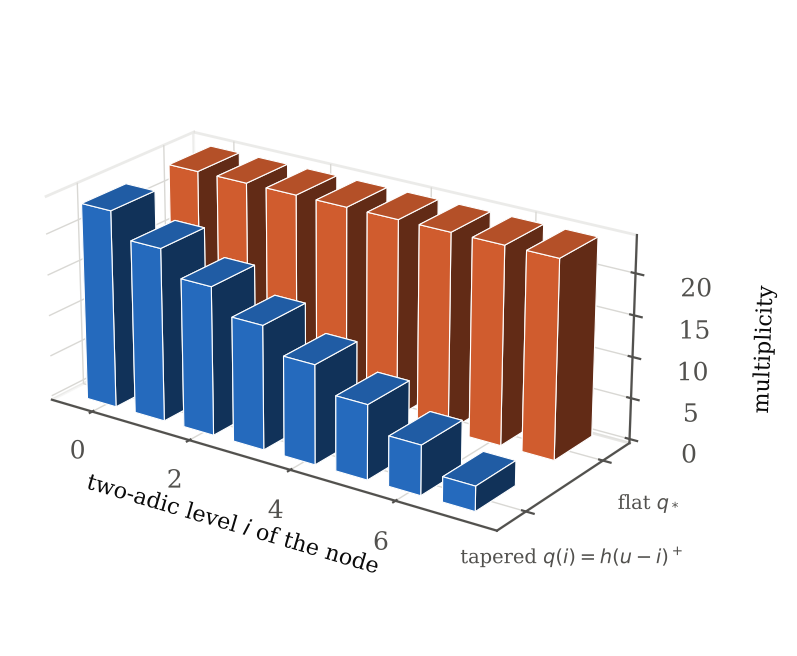
\includegraphics[width=0.8\textwidth]{fig_taper.png}
\caption{Multiplicities of the Hermite nodes by two-adic level, for $u=8$ and
$h=3$. The tapered choice $q(i)=h\max(0,u-i)$ of Lemma~\ref{lem:recovery}
(front) against a flat choice $q_*=hu$ on every level below $u$ (back). Both
give the odd points the multiplicity $hu$ that the degree count needs; only the
tapered one keeps the loss \eqref{eq:vEt} at $O(Dh)$.}\label{fig:taper}
\end{figure}

At a call of precision $p$ apply Lemma~\ref{lem:recovery} with the parameters
\eqref{eq:params}. For each $t$ with $q_t>0$ obtain the whole polynomial
$F(t+\alpha z)\bmod2^{p_t}$ by evaluating it at $M(2L-1)+1<s^4$ of the
interpolation points of Section~\ref{app:ring} and interpolating; the values
$F(t+\alpha\zeta)$ are computed in Section~\ref{app:modes} by child calls of
precision $p_t$. The precisions satisfy
\begin{equation}\label{eq:prec}
p\le s\lambda^{O(1)}2^{a_{d-1}},\qquad p_t=O_C(MD_t/u).
\end{equation}
The first bound holds at the root, where $p=P_0\le Cs$, and the increments
$8hD_t+8M(a+1)$ along a path are at most $s\lambda^{O(1)}2^{a_d}$ at depth $d$,
with $O(\log\lambda)$ depths. For the second, $q_t>0$ forces $i<u$, so
$D_t\ge2^{a_d-u}=2^{a_{d-1}+u}$; since $u\ge\lambda^{4/5}$, the factor $2^u$
exceeds every fixed power of $\lambda$, and both $p$ and $8M(a+1)$ are
$O(MD_t/u)$, as is $8hD_t$. All precisions are polynomial in $s$ because
$a\le4\varepsilon\lambda$.

\subsection{Modes for interactions between groups}\label{app:modes}
Fix $t$ with $i=\vtwo(t)<u$, put $D=L/2^i$, fix an interpolation point $\zeta$, and
work modulo $2^{p_t}$ with $T=t+\alpha\zeta$. Group the vertices on both sides by
their symbol in coordinate $i$; there are $r$ groups. Entries of $W(T)$ whose two
ports lie in the same group are \emph{local}.

The matrix $W(t)$ is local. Indeed $W_{xy}(t)=0$ unless $y=x+t$, and adding $t$,
whose lowest set bit is bit $i$, flips bit $i$ of the slot number. When the pair
of symbols of the packet in coordinate $i$ is unequal, bit $i$ of a slot
records the orientation, so a row slot and a column slot lie in the same group
exactly when their bits $i$ differ; when the pair is equal, the whole packet is
one group.

In a packet with unequal pair, write the column slots as $y=y_0+2^{i+1}j$ with
$0\le y_0<2^{i+1}$; the group of $y$ depends only on $y_0$, so these
\emph{tiles} are monochromatic. If a row $x$ and the tile of $y_0$ lie in
different groups, then $\vtwo(t-y_0+x)\le i$, for otherwise $y_0\equiv x+t\bmod
2^{i+1}$ and their bits $i$ would differ. The same holds with $T$ in place of $t$,
since $\vtwo(\alpha\zeta)>i$. Expanding geometrically,
\begin{equation}\label{eq:modes}
W_{xy}(T)\equiv\sum_{\substack{b\ge0\\ b+1<p_t}}
\frac{C(T)}{C'(0)(T-y_0+x)}\Bigl(\frac{2^{i+1}}{T-y_0+x}\Bigr)^bj^b
\pmod{2^{p_t}}.
\end{equation}
The first factor has valuation at least $a+1-i\ge1$ by the proof of
Lemma~\ref{lem:integral}, and the ratio has valuation at least one, so the term
of index $b$ is divisible by $2^{b+1}$ and the remainder of the geometric series
by $2^{p_t}$. For each packet, tile and $b$ introduce a \emph{mode} $Z$ of weight
$w_Z=b+1$, standing for
\[
L_Z(X)=\sum_{\text{real columns }y\text{ in the tile}}j^bX_y\qquad(j^0=1).
\]
Its \emph{source} is the group of the tile and its \emph{target} the other group
of the packet's pair. By \eqref{eq:modes}, each row form $(W(T)X)_x$ is its
local part plus a combination of the modes targeted at the group of $x$, with
coefficients divisible by $2^{w_Z}$. A packet has $2^{i+1}$ tiles, so there are at
most
\begin{equation}\label{eq:modecount}
\frac{3M}L\,2^{i+1}=\frac{6M}D
\end{equation}
modes of each weight.

Expand the product in \eqref{eq:F} as a polynomial in the modes. The coefficient
of a monomial $Z^\beta$ is divisible by $2^{\sum_Zw_Z\beta_Z}$, so modulo $2^{p_t}$
only the exponent vectors with
\begin{equation}\label{eq:budget}
\sum_Zw_Z\beta_Z<p_t
\end{equation}
contribute. Their number is $\exp(O(\sqrt{Mp_t/D}))=\exp(O_C(M/\sqrt u))$. Indeed,
for $\theta>0$ the generating function bounds the number by
\[
\exp\Bigl(\theta p_t+\frac{6M}D\sum_{j\ge1}-\ln(1-e^{-\theta j})\Bigr),\qquad
\sum_{j\ge1}-\ln(1-e^{-\theta j})=\sum_{h\ge1}\frac1{h(e^{\theta h}-1)}\le\frac{\pi^2}{6\theta},
\]
and $\theta=\sqrt{M/(Dp_t)}$ gives $\exp((1+\pi^2)\sqrt{Mp_t/D})$; then
\eqref{eq:prec} gives $\sqrt{Mp_t/D}=O(M/\sqrt u)$. The vectors are enumerated
with polynomial delay by choosing exponents one variable at a time within the
remaining budget.

\subsection{The child networks}\label{app:children}
For one vector $\beta$ satisfying \eqref{eq:budget} and one group $g\in[r]$, the
child network $\cN_{g,\beta}$ is built as follows. On one side put all current
vertices of group $g$, from both sides, with their ports and their lifted
entries reduced modulo $2^{p_t}$. On the other side put one vertex for each
packet, joined to every port of group $g$ in that packet; its ports are the row
bits $Y$ and column bits $X$ of group $g$ in the packet. Its tensor is the
coefficient of $\prod_ZZ^{\beta_Z}$, over the modes $Z$ of the packet targeted at
$g$, in the product of the row factors $l_{Y_x}$ of group $g$ in the packet,
written in the local column bits and the formal modes, multiplied by
$\prod_ZL_Z(X)^{\beta_Z}$ over the modes of the packet whose source is $g$. Empty
products are one; a positive exponent on a mode with no target rows, or on a
mode whose tile has no real column, gives zero.

Every mode has one source and one target, the coefficient extraction factors
over the groups of the rows, and the substitution of each mode uses only bits of
its source group. Distributing the product in \eqref{eq:F} and summing the bits
of each group independently therefore gives
\begin{equation}\label{eq:children}
F(t+\alpha\zeta)\equiv\sum_{\beta}\ \prod_{g=1}^rZ(\cN_{g,\beta})\pmod{2^{p_t}},
\end{equation}
the sum over the vectors satisfying \eqref{eq:budget}; the omitted monomials
vanish modulo $2^{p_t}$.

By Lemma~\ref{lem:packing}(3) a child has at most $6M/r=3M/32<M/8$ edges. Old
vertices keep their degrees, and a packet vertex has at most $2L\le\Delta$ ports,
so the invariants of Section~\ref{app:packing} hold inductively. A packet entry
is computed by expanding a product of at most $L$ affine factors, each with
polynomially many terms, in time $\exp(O(L\log s))=\exp(O(s^{9/10}))$ and
polynomial space; powers $L_Z(X)^{\beta_Z}$ are computed by repeated squaring. A
new tensor is described by its packet data, $\beta$, $\zeta$ and its creation
precision, and old tensors keep their descriptions, shared by reference, so
entry routines do not compose along the recursion.

\subsection{Proof of Theorem~\ref{thm:contraction}}\label{app:proof}
Embed the entries in $\cA_{P_0}$ and run the recursion. At an active call, for
every $t$ with $q_t>0$ and every interpolation point, compute
\eqref{eq:children} from the child contractions, interpolate $F(t+\alpha z)$,
and apply Lemma~\ref{lem:recovery}; at a leaf sum directly. Correctness follows
by induction from Lemmas~\ref{lem:integral} and~\ref{lem:recovery} and
\eqref{eq:children}.

A call has polynomially many nodes, points and groups, so by
\eqref{eq:budget} an active call at depth $d$ has at most
\[
s^{O(1)}\exp\Bigl(O_C\Bigl(\frac s{\sqrt\lambda}\Bigl(\frac{\sqrt2}8\Bigr)^d\Bigr)\Bigr)
\]
children, using $M\le Cs8^{-d}$ and $u_d=\Theta(\lambda/2^d)$. Over the
$O(\log\lambda)$ depths the number of calls is at most
$\exp(O_C(s/\sqrt\lambda)+O(\lambda\log\lambda))=\exp(O_C(s/\sqrt\lambda))$. A leaf
costs $2^H$ assignments with polynomially many entry evaluations each, that is
$\exp(O_C(H)+O_{C,A}(s^{9/10}))(s+L)^{O(1)}=\exp(O_{C,A}(s/\sqrt\lambda))(s+L)^{O(1)}$.
All other work is polynomial per generated term, which proves the time bound.
For space, traverse the recursion depth first, keeping at each of the
$O(\log\lambda)$ levels the Taylor data of the current call, its indices and its
new tensor descriptions, all of polynomial size by \eqref{eq:prec}. Finally read
off the coordinates of the result in $B_{P_0,\ell}$. \qed

%%==================================================================
\section{Programs that check the finite identities}\label{app:checks}
%%==================================================================

The archive contains a program written in Python with exact integer and
rational arithmetic. It builds the network $\cN(C)$ of
Section~\ref{sec:counting} for random circuits in $\cK(F,\beta)$ with all gate
kinds of Definition~\ref{def:gates}, including big weighted gates split into
blocks, and compares its contraction with exhaustive counting; it checks the
bounds of Lemma~\ref{lem:size} on the edges and degrees, the reduction of
Corollary~\ref{cor:ilp} on random zero-one programs, the identity
\eqref{eq:vEt} and the bound $\vtwo(E_t(0))\ge-6Dh$ for all admissible small
parameters, the integrality of Lemma~\ref{lem:integral}, the Hermite formula
\eqref{eq:hermite} on random polynomials, and the properties (1) to (3) of
Lemma~\ref{lem:packing} on random bipartite graphs with small parameters. For
the degree bound of Lemma~\ref{lem:size} it evaluates the largest possible
degree $\max\bigl(K+b,\lceil s/K\rceil b+1\bigr)$ for every $s$ up to
$3\cdot10^6$: the bound $\lceil s^{9/10}\rceil$ and the inequality $b\le K$ hold
for every $s\ge1416$, which is the constant of that lemma in this range. The
program runs in about twenty seconds and reports $27$ checks passed and none
failed. These checks confirm the finite statements; the proofs in the text do
not depend on them.

\section*{Declarations}

\subsection*{Data and code availability}
The sources of this paper, the catalogue of arXiv papers of
Section~\ref{sec:repositories} with the program that produced it, the list of
claims taken from Woeginger's page, and the program of
Appendix~\ref{app:checks} with its recorded output are archived at Zenodo,
\href{https://doi.org/\zenodoDOI}{doi:\zenodoDOI}.

\subsection*{Funding}
No funding was received for this work.

\subsection*{Competing interests}
The author has no competing interests to declare.

\subsection*{Ethics approval}
Not applicable. The work involves no human participants, animals or personal
data.

\subsection*{Use of artificial intelligence}
During the preparation of this work the author used Claude (Anthropic) to write
and run the programs of Appendix~\ref{app:checks} and of the literature
catalogue and to draft text. The author reviewed and edited the content and
takes full responsibility for the publication.

\subsection*{Acknowledgements}
The contraction theorem on which Theorem~A rests, and the proof reproduced in
Appendix~\ref{app:contraction}, are due to \oai{} \cite{OAI26}.

\FloatBarrier
\begingroup\raggedright\small
\begin{thebibliography}{CHOPRS22}
\bibitem[Aar16]{Aar16} S. Aaronson, \emph{$\mathsf P\overset{?}{=}\mathsf{NP}$}, in: Open Problems in Mathematics, J. F. Nash, Jr. and M. Th. Rassias (eds.), Springer, Cham, 2016, pp.~1--122. \href{https://doi.org/10.1007/978-3-319-32162-2_1}{doi:10.1007/978-3-319-32162-2\_1}
\bibitem[AB09]{AB09} S. Arora and B. Barak, \emph{Computational Complexity}, Cambridge University Press, Cambridge, 2009. \href{https://doi.org/10.1017/CBO9780511804090}{doi:10.1017/CBO9780511804090}
\bibitem[AB87]{AB87} N. Alon and R. B. Boppana, \emph{The monotone circuit complexity of boolean functions}, Combinatorica \textbf{7} (1987), no.~1, 1--22. \href{https://doi.org/10.1007/BF02579196}{doi:10.1007/BF02579196}
\bibitem[Ajt83]{Ajt83} M. Ajtai, \emph{$\Sigma^1_1$-formulae on finite structures}, Ann. Pure Appl. Logic \textbf{24} (1983), no.~1, 1--48. \href{https://doi.org/10.1016/0168-0072(83)90038-6}{doi:10.1016/0168-0072(83)90038-6}
\bibitem[AK10]{AK10} E. Allender and M. Kouck{\'y}, \emph{Amplifying lower bounds by means of self-reducibility}, J. ACM \textbf{57} (2010), no.~3, 1--36. \href{https://doi.org/10.1145/1706591.1706594}{doi:10.1145/1706591.1706594}
\bibitem[AKS04]{AKS04} M. Agrawal, N. Kayal and N. Saxena, \emph{PRIMES is in P}, Ann. of Math. (2) \textbf{160} (2004), no.~2, 781--793. \href{https://doi.org/10.4007/annals.2004.160.781}{doi:10.4007/annals.2004.160.781}
\bibitem[ALMSS98]{ALMSS98} S. Arora, C. Lund, R. Motwani, M. Sudan and M. Szegedy, \emph{Proof verification and the hardness of approximation problems}, J. ACM \textbf{45} (1998), no.~3, 501--555. \href{https://doi.org/10.1145/278298.278306}{doi:10.1145/278298.278306}
\bibitem[AS98]{AS98} S. Arora and S. Safra, \emph{Probabilistic checking of proofs}, J. ACM \textbf{45} (1998), no.~1, 70--122. \href{https://doi.org/10.1145/273865.273901}{doi:10.1145/273865.273901}
\bibitem[AW09]{AW09} S. Aaronson and A. Wigderson, \emph{Algebrization}, ACM Trans. Comput. Theory \textbf{1} (2009), no.~1, 1--54. \href{https://doi.org/10.1145/1490270.1490272}{doi:10.1145/1490270.1490272}
\bibitem[BGS75]{BGS75} T. Baker, J. Gill and R. Solovay, \emph{Relativizations of the $\mathcal P=?\mathcal{NP}$ question}, SIAM J. Comput. \textbf{4} (1975), no.~4, 431--442. \href{https://doi.org/10.1137/0204037}{doi:10.1137/0204037}
\bibitem[Bha26bsd]{Bha26bsd} D. Bhattacharjee, \emph{The $p$-primary part of the Tate--Shafarevich group in ranks three to six: paper, data and certificates}, Zenodo, release v1.0.2 (2026). \href{https://doi.org/10.5281/zenodo.23933270}{doi:10.5281/zenodo.23933270}
\bibitem[Bha26eth]{Bha26eth} D. Bhattacharjee, \emph{Source and verification code for the paper Subexponential Weighted Counting and Exact Optimisation}, Zenodo, release v1.4.0 (2026). \href{https://doi.org/10.5281/zenodo.23718560}{doi:10.5281/zenodo.23718560}
\bibitem[Bha26weil]{Bha26weil} D. Bhattacharjee, \emph{LaTeX source and verification code for the paper Algebraic Loci of Weil Classes on Abelian Varieties}, Zenodo, release v5.1.0 (2026). \href{https://doi.org/10.5281/zenodo.23227940}{doi:10.5281/zenodo.23227940}
\bibitem[BhaHex26]{BhaHex26} D. Bhattacharjee, \emph{Subexponential weighted counting and exact optimisation}, HexagonMath preprint 2610.00594v1 (2026), \url{https://hexagonmath.org/2610.00594v1}.
\bibitem[BIP19]{BIP19} P. B{\"u}rgisser, C. Ikenmeyer and G. Panova, \emph{No occurrence obstructions in geometric complexity theory}, J. Amer. Math. Soc. \textbf{32} (2019), no.~1, 163--193. \href{https://doi.org/10.1090/jams/908}{doi:10.1090/jams/908}
\bibitem[Blu84]{Blu84} N. Blum, \emph{A Boolean function requiring $3n$ network size}, Theoret. Comput. Sci. \textbf{28} (1984), no.~3, 337--345. \href{https://doi.org/10.1016/0304-3975(83)90029-4}{doi:10.1016/0304-3975(83)90029-4}
\bibitem[BSW01]{BSW01} E. Ben-Sasson and A. Wigderson, \emph{Short proofs are narrow---resolution made simple}, J. ACM \textbf{48} (2001), no.~2, 149--169. \href{https://doi.org/10.1145/375827.375835}{doi:10.1145/375827.375835}
\bibitem[Cai07]{Cai07} J.-Y. Cai, \emph{$\mathrm{S}_2^p\subseteq\mathrm{ZPP}^{\mathrm{NP}}$}, J. Comput. System Sci. \textbf{73} (2007), no.~1, 25--35. \href{https://doi.org/10.1016/j.jcss.2003.07.015}{doi:10.1016/j.jcss.2003.07.015}
\bibitem[Che11]{Che11} D. Yu. Cherukhin, \emph{Lower bounds for complexity of Boolean circuits of finite depth with arbitrary elements}, Discrete Math. Appl. \textbf{21} (2011), no.~4. \href{https://doi.org/10.1515/dma.2011.031}{doi:10.1515/dma.2011.031}
\bibitem[CHOPRS22]{CHOPRS22} L. Chen, S. Hirahara, I. C. Oliveira, J. Pich, N. Rajgopal and R. Santhanam, \emph{Beyond Natural Proofs: Hardness Magnification and Locality}, J. ACM \textbf{69} (2022), no.~4, 1--49. \href{https://doi.org/10.1145/3538391}{doi:10.1145/3538391}
\bibitem[CHR24]{CHR24} L. Chen, S. Hirahara and H. Ren, \emph{Symmetric Exponential Time Requires Near-Maximum Circuit Size}, in: Proceedings of the 56th Annual ACM Symposium on Theory of Computing (STOC 2024), 2024, pp.~1990--1999. \href{https://doi.org/10.1145/3618260.3649624}{doi:10.1145/3618260.3649624}
\bibitem[CIP06]{CIP06} C. Calabro, R. Impagliazzo and R. Paturi, \emph{A duality between clause width and clause density for SAT}, in: 21st Annual IEEE Conference on Computational Complexity (CCC 2006), 2006, pp.~252--260. \href{https://doi.org/10.1109/CCC.2006.6}{doi:10.1109/CCC.2006.6}
\bibitem[CIP09]{CIP09} C. Calabro, R. Impagliazzo and R. Paturi, \emph{The Complexity of Satisfiability of Small Depth Circuits}, in: Parameterized and Exact Computation (IWPEC 2009), Lecture Notes in Comput. Sci. \textbf{5917}, Springer, Berlin, 2009, pp.~75--85. \href{https://doi.org/10.1007/978-3-642-11269-0_6}{doi:10.1007/978-3-642-11269-0\_6}
\bibitem[CKKSZ15]{CKKSZ15} R. Chen, V. Kabanets, A. Kolokolova, R. Shaltiel and D. Zuckerman, \emph{Mining Circuit Lower Bound Proofs for Meta-Algorithms}, Comput. Complexity \textbf{24} (2015), no.~2, 333--392. \href{https://doi.org/10.1007/s00037-015-0100-0}{doi:10.1007/s00037-015-0100-0}
\bibitem[Clay]{Clay} Clay Mathematics Institute, \emph{P vs NP}, Millennium Prize Problems, official problem description by S. Cook, \url{https://www.claymath.org/millennium/p-vs-np/}.
\bibitem[Coo71]{Coo71} S. A. Cook, \emph{The complexity of theorem-proving procedures}, in: Proceedings of the Third Annual ACM Symposium on Theory of Computing (STOC 1971), 1971, pp.~151--158. \href{https://doi.org/10.1145/800157.805047}{doi:10.1145/800157.805047}
\bibitem[Coo73]{Coo73} S. A. Cook, \emph{A hierarchy for nondeterministic time complexity}, J. Comput. System Sci. \textbf{7} (1973), no.~4, 343--353. \href{https://doi.org/10.1016/S0022-0000(73)80028-5}{doi:10.1016/S0022-0000(73)80028-5}
\bibitem[CR79]{CR79} S. A. Cook and R. A. Reckhow, \emph{The relative efficiency of propositional proof systems}, J. Symbolic Logic \textbf{44} (1979), no.~1, 36--50. \href{https://doi.org/10.2307/2273702}{doi:10.2307/2273702}
\bibitem[CSS18]{CSS18} R. Chen, R. Santhanam and S. Srinivasan, \emph{Average-case lower bounds and satisfiability algorithms for small threshold circuits}, Theory Comput. \textbf{14} (2018), no.~1, 1--55. \href{https://doi.org/10.4086/toc.2018.v014a009}{doi:10.4086/toc.2018.v014a009}
\bibitem[Din07]{Din07} I. Dinur, \emph{The PCP theorem by gap amplification}, J. ACM \textbf{54} (2007), no.~3, Art.~12. \href{https://doi.org/10.1145/1236457.1236459}{doi:10.1145/1236457.1236459}
\bibitem[ECCC]{ECCC} Electronic Colloquium on Computational Complexity, \url{https://eccc.weizmann.ac.il/}.
\bibitem[Edm65]{Edm65} J. Edmonds, \emph{Paths, Trees, and Flowers}, Canad. J. Math. \textbf{17} (1965), 449--467. \href{https://doi.org/10.4153/CJM-1965-045-4}{doi:10.4153/CJM-1965-045-4}
\bibitem[FGHK16]{FGHK16} M. G. Find, A. Golovnev, E. A. Hirsch and A. S. Kulikov, \emph{A better-than-$3n$ lower bound for the circuit complexity of an explicit function}, in: 57th Annual IEEE Symposium on Foundations of Computer Science (FOCS 2016), 2016, pp.~89--98. \href{https://doi.org/10.1109/FOCS.2016.19}{doi:10.1109/FOCS.2016.19}
\bibitem[FLMV05]{FLMV05} L. Fortnow, R. Lipton, D. van Melkebeek and A. Viglas, \emph{Time-space lower bounds for satisfiability}, J. ACM \textbf{52} (2005), no.~6, 835--865. \href{https://doi.org/10.1145/1101821.1101822}{doi:10.1145/1101821.1101822}
\bibitem[For09]{For09} L. Fortnow, \emph{The status of the P versus NP problem}, Commun. ACM \textbf{52} (2009), no.~9, 78--86. \href{https://doi.org/10.1145/1562164.1562186}{doi:10.1145/1562164.1562186}
\bibitem[FSS84]{FSS84} M. Furst, J. B. Saxe and M. Sipser, \emph{Parity, circuits, and the polynomial-time hierarchy}, Math. Systems Theory \textbf{17} (1984), no.~1, 13--27. \href{https://doi.org/10.1007/BF01744431}{doi:10.1007/BF01744431}
\bibitem[Gas19]{Gas19} W. I. Gasarch, \emph{Guest column: the third P $=?$ NP poll}, ACM SIGACT News \textbf{50} (2019), no.~1, 38--59. \href{https://doi.org/10.1145/3319627.3319636}{doi:10.1145/3319627.3319636}
\bibitem[GHKK18]{GHKK18} A. Golovnev, E. A. Hirsch, A. Knop and A. S. Kulikov, \emph{On the limits of gate elimination}, J. Comput. System Sci. \textbf{96} (2018), 107--119. \href{https://doi.org/10.1016/j.jcss.2018.04.005}{doi:10.1016/j.jcss.2018.04.005}
\bibitem[GJ79]{GJ79} M. R. Garey and D. S. Johnson, \emph{Computers and Intractability: A Guide to the Theory of NP-Completeness}, W. H. Freeman, San Francisco, 1979.
\bibitem[GKST18]{GKST18} A. Golovnev, A. S. Kulikov, A. V. Smal and S. Tamaki, \emph{Gate elimination: circuit size lower bounds and \#SAT upper bounds}, Theoret. Comput. Sci. \textbf{719} (2018), 46--63. \href{https://doi.org/10.1016/j.tcs.2017.11.008}{doi:10.1016/j.tcs.2017.11.008}
\bibitem[Hak85]{Hak85} A. Haken, \emph{The intractability of resolution}, Theoret. Comput. Sci. \textbf{39} (1985), 297--308. \href{https://doi.org/10.1016/0304-3975(85)90144-6}{doi:10.1016/0304-3975(85)90144-6}
\bibitem[Has86]{Has86} J. H{\aa}stad, \emph{Almost optimal lower bounds for small depth circuits}, in: Proceedings of the 18th Annual ACM Symposium on Theory of Computing (STOC 1986), 1986, pp.~6--20. \href{https://doi.org/10.1145/12130.12132}{doi:10.1145/12130.12132}
\bibitem[Has98]{Has98} J. H{\aa}stad, \emph{The shrinkage exponent of de Morgan formulas is $2$}, SIAM J. Comput. \textbf{27} (1998), no.~1, 48--64. \href{https://doi.org/10.1137/S0097539794261556}{doi:10.1137/S0097539794261556}
\bibitem[Her14]{Her14} T. Hertli, \emph{3-SAT faster and simpler---Unique-SAT bounds for PPSZ hold in general}, SIAM J. Comput. \textbf{43} (2014), no.~2, 718--729. \href{https://doi.org/10.1137/120868177}{doi:10.1137/120868177}
\bibitem[Hir18]{Hir18} S. Hirahara, \emph{Non-Black-Box Worst-Case to Average-Case Reductions within NP}, in: 59th Annual IEEE Symposium on Foundations of Computer Science (FOCS 2018), 2018, pp.~247--258. \href{https://doi.org/10.1109/FOCS.2018.00032}{doi:10.1109/FOCS.2018.00032}
\bibitem[Hir22]{Hir22} S. Hirahara, \emph{NP-hardness of learning programs and partial MCSP}, in: 63rd Annual IEEE Symposium on Foundations of Computer Science (FOCS 2022), 2022, pp.~968--979. \href{https://doi.org/10.1109/FOCS54457.2022.00095}{doi:10.1109/FOCS54457.2022.00095}
\bibitem[HMPST93]{HMPST93} A. Hajnal, W. Maass, P. Pudl{\'a}k, M. Szegedy and G. Tur{\'a}n, \emph{Threshold circuits of bounded depth}, J. Comput. System Sci. \textbf{46} (1993), no.~2, 129--154. \href{https://doi.org/10.1016/0022-0000(93)90001-D}{doi:10.1016/0022-0000(93)90001-D}
\bibitem[HPV77]{HPV77} J. Hopcroft, W. Paul and L. Valiant, \emph{On Time Versus Space}, J. ACM \textbf{24} (1977), no.~2, 332--337. \href{https://doi.org/10.1145/322003.322015}{doi:10.1145/322003.322015}
\bibitem[HS65]{HS65} J. Hartmanis and R. E. Stearns, \emph{On the computational complexity of algorithms}, Trans. Amer. Math. Soc. \textbf{117} (1965), 285--306. \href{https://doi.org/10.1090/S0002-9947-1965-0170805-7}{doi:10.1090/S0002-9947-1965-0170805-7}
\bibitem[IKW02]{IKW02} R. Impagliazzo, V. Kabanets and A. Wigderson, \emph{In search of an easy witness: exponential time vs.\ probabilistic polynomial time}, J. Comput. System Sci. \textbf{65} (2002), no.~4, 672--694. \href{https://doi.org/10.1016/S0022-0000(02)00024-7}{doi:10.1016/S0022-0000(02)00024-7}
\bibitem[ILPS14]{ILPS14} R. Impagliazzo, S. Lovett, R. Paturi and S. Schneider, \emph{0-1 integer linear programming with a linear number of constraints}, preprint (2014), \href{https://arxiv.org/abs/1401.5512}{arXiv:1401.5512}.
\bibitem[ILW23]{ILW23} R. Ilango, J. Li and R. R. Williams, \emph{Indistinguishability obfuscation, range avoidance, and bounded arithmetic}, in: Proceedings of the 55th Annual ACM Symposium on Theory of Computing (STOC 2023), 2023, pp.~1076--1089. \href{https://doi.org/10.1145/3564246.3585187}{doi:10.1145/3564246.3585187}
\bibitem[IM02]{IM02} K. Iwama and H. Morizumi, \emph{An explicit lower bound of $5n-o(n)$ for Boolean circuits}, in: Mathematical Foundations of Computer Science 2002, Lecture Notes in Comput. Sci. \textbf{2420}, Springer, Berlin, 2002, pp.~353--364. \href{https://doi.org/10.1007/3-540-45687-2_29}{doi:10.1007/3-540-45687-2\_29}
\bibitem[Imp95]{Imp95} R. Impagliazzo, \emph{A personal view of average-case complexity}, in: Proceedings of the Tenth Annual Structure in Complexity Theory Conference, IEEE, 1995, pp.~134--147. \href{https://doi.org/10.1109/SCT.1995.514853}{doi:10.1109/SCT.1995.514853}
\bibitem[IP01]{IP01} R. Impagliazzo and R. Paturi, \emph{On the complexity of $k$-SAT}, J. Comput. System Sci. \textbf{62} (2001), no.~2, 367--375. \href{https://doi.org/10.1006/jcss.2000.1727}{doi:10.1006/jcss.2000.1727}
\bibitem[IPS13]{IPS13} R. Impagliazzo, R. Paturi and S. Schneider, \emph{A Satisfiability Algorithm for Sparse Depth Two Threshold Circuits}, in: 54th Annual IEEE Symposium on Foundations of Computer Science (FOCS 2013), 2013, pp.~479--488. \href{https://doi.org/10.1109/FOCS.2013.58}{doi:10.1109/FOCS.2013.58}
\bibitem[IPS97]{IPS97} R. Impagliazzo, R. Paturi and M. E. Saks, \emph{Size--Depth Tradeoffs for Threshold Circuits}, SIAM J. Comput. \textbf{26} (1997), no.~3, 693--707. \href{https://doi.org/10.1137/S0097539792282965}{doi:10.1137/S0097539792282965}
\bibitem[IPZ01]{IPZ01} R. Impagliazzo, R. Paturi and F. Zane, \emph{Which Problems Have Strongly Exponential Complexity?}, J. Comput. System Sci. \textbf{63} (2001), no.~4, 512--530. \href{https://doi.org/10.1006/jcss.2001.1774}{doi:10.1006/jcss.2001.1774}
\bibitem[IW97]{IW97} R. Impagliazzo and A. Wigderson, \emph{$P=BPP$ if $E$ requires exponential circuits: derandomizing the XOR lemma}, in: Proceedings of the 29th Annual ACM Symposium on Theory of Computing (STOC 1997), 1997, pp.~220--229. \href{https://doi.org/10.1145/258533.258590}{doi:10.1145/258533.258590}
\bibitem[JMV15]{JMV15} H. Jahanjou, E. Miles and E. Viola, \emph{Local Reductions}, in: Automata, Languages, and Programming (ICALP 2015), Part I, Lecture Notes in Comput. Sci. \textbf{9134}, Springer, Berlin, 2015, pp.~749--760. \href{https://doi.org/10.1007/978-3-662-47672-7_61}{doi:10.1007/978-3-662-47672-7\_61}
\bibitem[Juk10]{Juk10} S. Jukna, \emph{Representing (0, 1)-matrices by boolean circuits}, Discrete Math. \textbf{310} (2010), no.~1, 184--187. \href{https://doi.org/10.1016/j.disc.2009.07.011}{doi:10.1016/j.disc.2009.07.011}
\bibitem[Juk12]{Juk12} S. Jukna, \emph{Boolean Function Complexity}, Algorithms Combin. \textbf{27}, Springer, Heidelberg, 2012. \href{https://doi.org/10.1007/978-3-642-24508-4}{doi:10.1007/978-3-642-24508-4}
\bibitem[Kan82]{Kan82} R. Kannan, \emph{Circuit-size lower bounds and non-reducibility to sparse sets}, Inform. and Control \textbf{55} (1982), no.~1-3, 40--56. \href{https://doi.org/10.1016/S0019-9958(82)90382-5}{doi:10.1016/S0019-9958(82)90382-5}
\bibitem[Kar72]{Kar72} R. M. Karp, \emph{Reducibility among Combinatorial Problems}, in: Complexity of Computer Computations, R. E. Miller and J. W. Thatcher (eds.), Plenum Press, New York, 1972, pp.~85--103. \href{https://doi.org/10.1007/978-1-4684-2001-2_9}{doi:10.1007/978-1-4684-2001-2\_9}
\bibitem[KC00]{KC00} V. Kabanets and J.-Y. Cai, \emph{Circuit minimization problem}, in: Proceedings of the 32nd Annual ACM Symposium on Theory of Computing (STOC 2000), 2000, pp.~73--79. \href{https://doi.org/10.1145/335305.335314}{doi:10.1145/335305.335314}
\bibitem[KI04]{KI04} V. Kabanets and R. Impagliazzo, \emph{Derandomizing Polynomial Identity Tests Means Proving Circuit Lower Bounds}, Comput. Complexity \textbf{13} (2004), no.~1-2, 1--46. \href{https://doi.org/10.1007/s00037-004-0182-6}{doi:10.1007/s00037-004-0182-6}
\bibitem[Kor21]{Kor21} O. Korten, \emph{The hardest explicit construction}, in: 62nd Annual IEEE Symposium on Foundations of Computer Science (FOCS 2021), 2021, pp.~433--444. \href{https://doi.org/10.1109/FOCS52979.2021.00051}{doi:10.1109/FOCS52979.2021.00051}
\bibitem[Kra19]{Kra19} J. Kraj{\'\i}{\v c}ek, \emph{Proof Complexity}, Encyclopedia Math. Appl. \textbf{170}, Cambridge University Press, Cambridge, 2019. \href{https://doi.org/10.1017/9781108242066}{doi:10.1017/9781108242066}
\bibitem[KW16]{KW16} D. M. Kane and R. Williams, \emph{Super-linear gate and super-quadratic wire lower bounds for depth-two and depth-three threshold circuits}, in: Proceedings of the 48th Annual ACM Symposium on Theory of Computing (STOC 2016), 2016, pp.~633--643. \href{https://doi.org/10.1145/2897518.2897636}{doi:10.1145/2897518.2897636}
\bibitem[KW90]{KW90} M. Karchmer and A. Wigderson, \emph{Monotone Circuits for Connectivity Require Super-Logarithmic Depth}, SIAM J. Discrete Math. \textbf{3} (1990), no.~2, 255--265. \href{https://doi.org/10.1137/0403021}{doi:10.1137/0403021}
\bibitem[Lad75]{Lad75} R. E. Ladner, \emph{On the Structure of Polynomial Time Reducibility}, J. ACM \textbf{22} (1975), no.~1, 155--171. \href{https://doi.org/10.1145/321864.321877}{doi:10.1145/321864.321877}
\bibitem[Lev73]{Lev73} L. A. Levin, \emph{Universal sequential search problems}, Problemy Peredachi Informatsii \textbf{9} (1973), no.~3, 115--116 (in Russian); English translation in Problems Inform. Transmission \textbf{9} (1973), 265--266.
\bibitem[Li24]{Li24} Z. Li, \emph{Symmetric Exponential Time Requires Near-Maximum Circuit Size: Simplified, Truly Uniform}, in: Proceedings of the 56th Annual ACM Symposium on Theory of Computing (STOC 2024), 2024, pp.~2000--2007. \href{https://doi.org/10.1145/3618260.3649615}{doi:10.1145/3618260.3649615}
\bibitem[LST21]{LST21} N. Limaye, S. Srinivasan and S. Tavenas, \emph{Superpolynomial Lower Bounds Against Low-Depth Algebraic Circuits}, in: 62nd Annual IEEE Symposium on Foundations of Computer Science (FOCS 2021), 2021, pp.~804--814. \href{https://doi.org/10.1109/FOCS52979.2021.00083}{doi:10.1109/FOCS52979.2021.00083}
\bibitem[LY22]{LY22} J. Li and T. Yang, \emph{$3.1n-o(n)$ circuit lower bounds for explicit functions}, in: Proceedings of the 54th Annual ACM Symposium on Theory of Computing (STOC 2022), 2022, pp.~1180--1193. \href{https://doi.org/10.1145/3519935.3519976}{doi:10.1145/3519935.3519976}
\bibitem[MS01]{MS01} K. D. Mulmuley and M. Sohoni, \emph{Geometric complexity theory I: an approach to the P vs.\ NP and related problems}, SIAM J. Comput. \textbf{31} (2001), no.~2, 496--526. \href{https://doi.org/10.1137/S009753970038715X}{doi:10.1137/S009753970038715X}
\bibitem[MS08]{MS08} I. L. Markov and Y. Shi, \emph{Simulating Quantum Computation by Contracting Tensor Networks}, SIAM J. Comput. \textbf{38} (2008), no.~3, 963--981. \href{https://doi.org/10.1137/050644756}{doi:10.1137/050644756}
\bibitem[Mul12]{Mul12} K. D. Mulmuley, \emph{The GCT program toward the P vs.\ NP problem}, Commun. ACM \textbf{55} (2012), no.~6, 98--107. \href{https://doi.org/10.1145/2184319.2184341}{doi:10.1145/2184319.2184341}
\bibitem[MW20]{MW20} C. D. Murray and R. R. Williams, \emph{Circuit lower bounds for nondeterministic quasi-polytime from a new easy witness lemma}, SIAM J. Comput. \textbf{49} (2020), no.~5, STOC18-300--STOC18-322. \href{https://doi.org/10.1137/18M1195887}{doi:10.1137/18M1195887}
\bibitem[NW94]{NW94} N. Nisan and A. Wigderson, \emph{Hardness vs randomness}, J. Comput. System Sci. \textbf{49} (1994), no.~2, 149--167. \href{https://doi.org/10.1016/S0022-0000(05)80043-1}{doi:10.1016/S0022-0000(05)80043-1}
\bibitem[OAI26]{OAI26} OpenAI, \emph{The exponential time hypothesis is false}, preprint, 25 October 2026, \url{https://github.com/openai/math/blob/main/preprints/The-Exponential-Time-Hypothesis-is-False-October-25-2026/paper.pdf}.
\bibitem[OS18]{OS18} I. C. Oliveira and R. Santhanam, \emph{Hardness Magnification for Natural Problems}, in: 59th Annual IEEE Symposium on Foundations of Computer Science (FOCS 2018), 2018, pp.~65--76. \href{https://doi.org/10.1109/FOCS.2018.00016}{doi:10.1109/FOCS.2018.00016}
\bibitem[PPST83]{PPST83} W. J. Paul, N. Pippenger, E. Szemeredi and W. T. Trotter, \emph{On determinism versus non-determinism and related problems}, in: 24th Annual Symposium on Foundations of Computer Science (FOCS 1983), IEEE, 1983, pp.~429--438. \href{https://doi.org/10.1109/SFCS.1983.39}{doi:10.1109/SFCS.1983.39}
\bibitem[PPSZ05]{PPSZ05} R. Paturi, P. Pudl{\'a}k, M. E. Saks and F. Zane, \emph{An improved exponential-time algorithm for $k$-SAT}, J. ACM \textbf{52} (2005), no.~3, 337--364. \href{https://doi.org/10.1145/1066100.1066101}{doi:10.1145/1066100.1066101}
\bibitem[Pud94]{Pud94} P. Pudl{\'a}k, \emph{Communication in bounded depth circuits}, Combinatorica \textbf{14} (1994), no.~2, 203--216. \href{https://doi.org/10.1007/BF01215351}{doi:10.1007/BF01215351}
\bibitem[Rag88]{Rag88} P. Raghavan, \emph{Probabilistic construction of deterministic algorithms: Approximating packing integer programs}, J. Comput. System Sci. \textbf{37} (1988), no.~2, 130--143. \href{https://doi.org/10.1016/0022-0000(88)90003-7}{doi:10.1016/0022-0000(88)90003-7}
\bibitem[Raz87]{Raz87} A. A. Razborov, \emph{Lower bounds on the size of bounded depth circuits over a complete basis with logical addition}, Math. Notes Acad. Sci. USSR \textbf{41} (1987), no.~4, 333--338. \href{https://doi.org/10.1007/BF01137685}{doi:10.1007/BF01137685}
\bibitem[RM99]{RM99} R. Raz and P. McKenzie, \emph{Separation of the Monotone NC Hierarchy}, Combinatorica \textbf{19} (1999), no.~3, 403--435. \href{https://doi.org/10.1007/s004930050062}{doi:10.1007/s004930050062}
\bibitem[Ros08]{Ros08} B. Rossman, \emph{On the constant-depth complexity of $k$-clique}, in: Proceedings of the 40th Annual ACM Symposium on Theory of Computing (STOC 2008), 2008, pp.~721--730. \href{https://doi.org/10.1145/1374376.1374480}{doi:10.1145/1374376.1374480}
\bibitem[RR97]{RR97} A. A. Razborov and S. Rudich, \emph{Natural Proofs}, J. Comput. System Sci. \textbf{55} (1997), no.~1, 24--35. \href{https://doi.org/10.1006/jcss.1997.1494}{doi:10.1006/jcss.1997.1494}
\bibitem[RSW22]{RSW22} H. Ren, R. Santhanam and Z. Wang, \emph{On the range avoidance problem for circuits}, in: 63rd Annual IEEE Symposium on Foundations of Computer Science (FOCS 2022), 2022, pp.~640--650. \href{https://doi.org/10.1109/FOCS54457.2022.00067}{doi:10.1109/FOCS54457.2022.00067}
\bibitem[RTS00]{RTS00} J. Radhakrishnan and A. Ta-Shma, \emph{Bounds for Dispersers, Extractors, and Depth-Two Superconcentrators}, SIAM J. Discrete Math. \textbf{13} (2000), no.~1, 2--24. \href{https://doi.org/10.1137/S0895480197329508}{doi:10.1137/S0895480197329508}
\bibitem[San09]{San09} R. Santhanam, \emph{Circuit Lower Bounds for Merlin--Arthur Classes}, SIAM J. Comput. \textbf{39} (2009), no.~3, 1038--1061. \href{https://doi.org/10.1137/070702680}{doi:10.1137/070702680}
\bibitem[San10]{San10} R. Santhanam, \emph{Fighting Perebor: New and Improved Algorithms for Formula and QBF Satisfiability}, in: 51st Annual IEEE Symposium on Foundations of Computer Science (FOCS 2010), 2010, pp.~183--192. \href{https://doi.org/10.1109/FOCS.2010.25}{doi:10.1109/FOCS.2010.25}
\bibitem[Sav70]{Sav70} W. J. Savitch, \emph{Relationships between nondeterministic and deterministic tape complexities}, J. Comput. System Sci. \textbf{4} (1970), no.~2, 177--192. \href{https://doi.org/10.1016/S0022-0000(70)80006-X}{doi:10.1016/S0022-0000(70)80006-X}
\bibitem[Sch80]{Sch80} C. Schnorr, \emph{A $3n$-lower bound on the network complexity of Boolean functions}, Theoret. Comput. Sci. \textbf{10} (1980), no.~1, 83--92. \href{https://doi.org/10.1016/0304-3975(80)90074-2}{doi:10.1016/0304-3975(80)90074-2}
\bibitem[Sch99]{Sch99} U. Sch{\"o}ning, \emph{A probabilistic algorithm for $k$-SAT and constraint satisfaction problems}, in: 40th Annual Symposium on Foundations of Computer Science (FOCS 1999), IEEE, 1999, pp.~410--414. \href{https://doi.org/10.1109/SFFCS.1999.814612}{doi:10.1109/SFFCS.1999.814612}
\bibitem[SFM78]{SFM78} J. I. Seiferas, M. J. Fischer and A. R. Meyer, \emph{Separating Nondeterministic Time Complexity Classes}, J. ACM \textbf{25} (1978), no.~1, 146--167. \href{https://doi.org/10.1145/322047.322061}{doi:10.1145/322047.322061}
\bibitem[Sha49]{Sha49} C. E. Shannon, \emph{The Synthesis of Two-Terminal Switching Circuits}, Bell System Tech. J. \textbf{28} (1949), no.~1, 59--98. \href{https://doi.org/10.1002/j.1538-7305.1949.tb03624.x}{doi:10.1002/j.1538-7305.1949.tb03624.x}
\bibitem[Sip92]{Sip92} M. Sipser, \emph{The history and status of the P versus NP question}, in: Proceedings of the 24th Annual ACM Symposium on Theory of Computing (STOC 1992), 1992, pp.~603--618. \href{https://doi.org/10.1145/129712.129771}{doi:10.1145/129712.129771}
\bibitem[Smo87]{Smo87} R. Smolensky, \emph{Algebraic methods in the theory of lower bounds for Boolean circuit complexity}, in: Proceedings of the 19th Annual ACM Symposium on Theory of Computing (STOC 1987), 1987, pp.~77--82. \href{https://doi.org/10.1145/28395.28404}{doi:10.1145/28395.28404}
\bibitem[ST13]{ST13} K. Seto and S. Tamaki, \emph{A satisfiability algorithm and average-case hardness for formulas over the full binary basis}, Comput. Complexity \textbf{22} (2013), no.~2, 245--274. \href{https://doi.org/10.1007/s00037-013-0067-7}{doi:10.1007/s00037-013-0067-7}
\bibitem[Tal14]{Tal14} A. Tal, \emph{Shrinkage of de Morgan formulae by spectral techniques}, in: 55th Annual IEEE Symposium on Foundations of Computer Science (FOCS 2014), 2014, pp.~551--560. \href{https://doi.org/10.1109/FOCS.2014.65}{doi:10.1109/FOCS.2014.65}
\bibitem[Tar88]{Tar88} {\'E}. Tardos, \emph{The gap between monotone and non-monotone circuit complexity is exponential}, Combinatorica \textbf{8} (1988), no.~1, 141--142. \href{https://doi.org/10.1007/BF02122563}{doi:10.1007/BF02122563}
\bibitem[Tod91]{Tod91} S. Toda, \emph{PP is as hard as the polynomial-time hierarchy}, SIAM J. Comput. \textbf{20} (1991), no.~5, 865--877. \href{https://doi.org/10.1137/0220053}{doi:10.1137/0220053}
\bibitem[Val77]{Val77} L. G. Valiant, \emph{Graph-theoretic arguments in low-level complexity}, in: Mathematical Foundations of Computer Science 1977, Lecture Notes in Comput. Sci. \textbf{53}, Springer, Berlin, 1977, pp.~162--176. \href{https://doi.org/10.1007/3-540-08353-7_135}{doi:10.1007/3-540-08353-7\_135}
\bibitem[Val79a]{Val79a} L. G. Valiant, \emph{Completeness classes in algebra}, in: Proceedings of the 11th Annual ACM Symposium on Theory of Computing (STOC 1979), 1979, pp.~249--261. \href{https://doi.org/10.1145/800135.804419}{doi:10.1145/800135.804419}
\bibitem[Val79b]{Val79b} L. Valiant, \emph{The complexity of computing the permanent}, Theoret. Comput. Sci. \textbf{8} (1979), no.~2, 189--201. \href{https://doi.org/10.1016/0304-3975(79)90044-6}{doi:10.1016/0304-3975(79)90044-6}
\bibitem[vzGG13]{vzGG13} J. von zur Gathen and J. Gerhard, \emph{Modern Computer Algebra}, third edition, Cambridge University Press, Cambridge, 2013. \href{https://doi.org/10.1017/CBO9781139856065}{doi:10.1017/CBO9781139856065}
\bibitem[Wig19]{Wig19} A. Wigderson, \emph{Mathematics and Computation: A Theory Revolutionizing Technology and Science}, Princeton University Press, Princeton, 2019.
\bibitem[Wil05]{Wil05} R. Williams, \emph{A new algorithm for optimal 2-constraint satisfaction and its implications}, Theoret. Comput. Sci. \textbf{348} (2005), no.~2-3, 357--365. \href{https://doi.org/10.1016/j.tcs.2005.09.023}{doi:10.1016/j.tcs.2005.09.023}
\bibitem[Wil13]{Wil13} R. Williams, \emph{Improving exhaustive search implies superpolynomial lower bounds}, SIAM J. Comput. \textbf{42} (2013), no.~3, 1218--1244. \href{https://doi.org/10.1137/10080703X}{doi:10.1137/10080703X}
\bibitem[Wil14]{Wil14} R. Williams, \emph{Nonuniform ACC circuit lower bounds}, J. ACM \textbf{61} (2014), no.~1, 1--32. \href{https://doi.org/10.1145/2559903}{doi:10.1145/2559903}
\bibitem[Wil14b]{Wil14b} R. Williams, \emph{New algorithms and lower bounds for circuits with linear threshold gates}, in: Proceedings of the 46th Annual ACM Symposium on Theory of Computing (STOC 2014), 2014, pp.~194--202. \href{https://doi.org/10.1145/2591796.2591858}{doi:10.1145/2591796.2591858}
\bibitem[Wil14c]{Wil14c} R. Williams, \emph{Algorithms for Circuits and Circuits for Algorithms}, in: 29th IEEE Conference on Computational Complexity (CCC 2014), 2014, pp.~248--261. \href{https://doi.org/10.1109/CCC.2014.33}{doi:10.1109/CCC.2014.33}
\bibitem[Wil16]{Wil16} R. R. Williams, \emph{Natural Proofs versus Derandomization}, SIAM J. Comput. \textbf{45} (2016), no.~2, 497--529. \href{https://doi.org/10.1137/130938219}{doi:10.1137/130938219}
\bibitem[Wil25]{Wil25} R. R. Williams, \emph{Simulating Time with Square-Root Space}, in: Proceedings of the 57th Annual ACM Symposium on Theory of Computing (STOC 2025), 2025, pp.~13--23. \href{https://doi.org/10.1145/3717823.3718225}{doi:10.1145/3717823.3718225}
\bibitem[Woe16]{Woe16} G. J. Woeginger, \emph{The P-versus-NP page}, \url{https://wscor.win.tue.nl/woeginger/P-versus-NP.htm}, last updated 2016.
\bibitem[Yan91]{Yan91} M. Yannakakis, \emph{Expressing combinatorial optimization problems by linear programs}, J. Comput. System Sci. \textbf{43} (1991), no.~3, 441--466. \href{https://doi.org/10.1016/0022-0000(91)90024-Y}{doi:10.1016/0022-0000(91)90024-Y}
\bibitem[Yao85]{Yao85} A. C.-C. Yao, \emph{Separating the polynomial-time hierarchy by oracles}, in: 26th Annual Symposium on Foundations of Computer Science (FOCS 1985), IEEE, 1985, pp.~1--10. \href{https://doi.org/10.1109/SFCS.1985.49}{doi:10.1109/SFCS.1985.49}
\bibitem[Zak83]{Zak83} S. {\v Z}{\'a}k, \emph{A Turing machine time hierarchy}, Theoret. Comput. Sci. \textbf{26} (1983), no.~3, 327--333. \href{https://doi.org/10.1016/0304-3975(83)90015-4}{doi:10.1016/0304-3975(83)90015-4}
\bibitem[Zoo]{Zoo} S. Aaronson et al., \emph{The Complexity Zoo}, \url{https://complexityzoo.net/Complexity_Zoo}.
\end{thebibliography}
\endgroup

\end{document}
